% !TeX spellcheck = pl_PL
% 
\newpage\section{Projekt systemu \textsl{\NazwaSys}}\label{sec:projekt}
Głównym celem pracy dyplomowej jest zaprojektowanie systemu. Opisywany rozdział dokładnie przedstawi projekt kompletnego systemu. Punkt \ref{sec:Diagramy UML} obrazuje na diagramach UML przypadki użycia poszczególnych funkcjonalności urządzeń, następnie wyszczególnione zostaną sekwencje działań głównych funkcji systemu oraz przedstawione zostaną modele bazy danych i wszystkich klas wyszczególnione dla każdego urządzenia osobno. 

Podrozdział \ref{sec:Schemat elektryczny zamka} zawiera uproszczony schemat elektryczny urządzenia sterującego zamkami. Następnie przedstawiona zostanie komunikacja modułów z aplikacją serwerową, tzn. opisane zostanie API serwera pozwalające podłączenie innych urządzeń do systemu oraz przebieg transmisji danych pomiędzy urządzeniem sterującym a aplikacją mobilną.

Punkt \ref{sec:Projekt interfejsu graficznego} przedstawia projekt interfejsu graficznego, wraz z objaśnieniami zastosowanej kolorystyki i symboli.

Ostatni rozdział opisuje mechanizmy bezpieczeństwa zaprojektowane w systemie z uwzględnieniem głównych właściwości poufności, integralności oraz dostępności.

\subsection{Diagramy UML}\label{sec:Diagramy UML}
Podrozdział zawiera projekt systemu w postaci diagramów UML. W pierwszej kolejności przedstawiony zostanie diagram przypadków użycia, gdzie wymienione zostaną wszystkie funkcjonalności systemu oraz przyłączone do nich zostaną poszczególne podmioty (aktorzy) systemu, które biorą udział przy wykonywaniu danej funkcjonalności. Następnie omówiony zostanie diagram relacji oraz encji bazy danych. Na koniec omówione zostaną diagramy klas, wykonane dla każdego modułu osobno. 
	\subsubsection[Diagram przypadków użycia]{Diagram przypadków użycia [Maciej Marciniak]}
	Diagram przypadków użycia (funkcjonalności) systemu wraz z opowiadającymi aktorami przedstawiono na Rys. \ref{diagram:diagram przypadków_użycia}.
	\begin{landscape}
		\begin{figure}[!h]
			\centering
			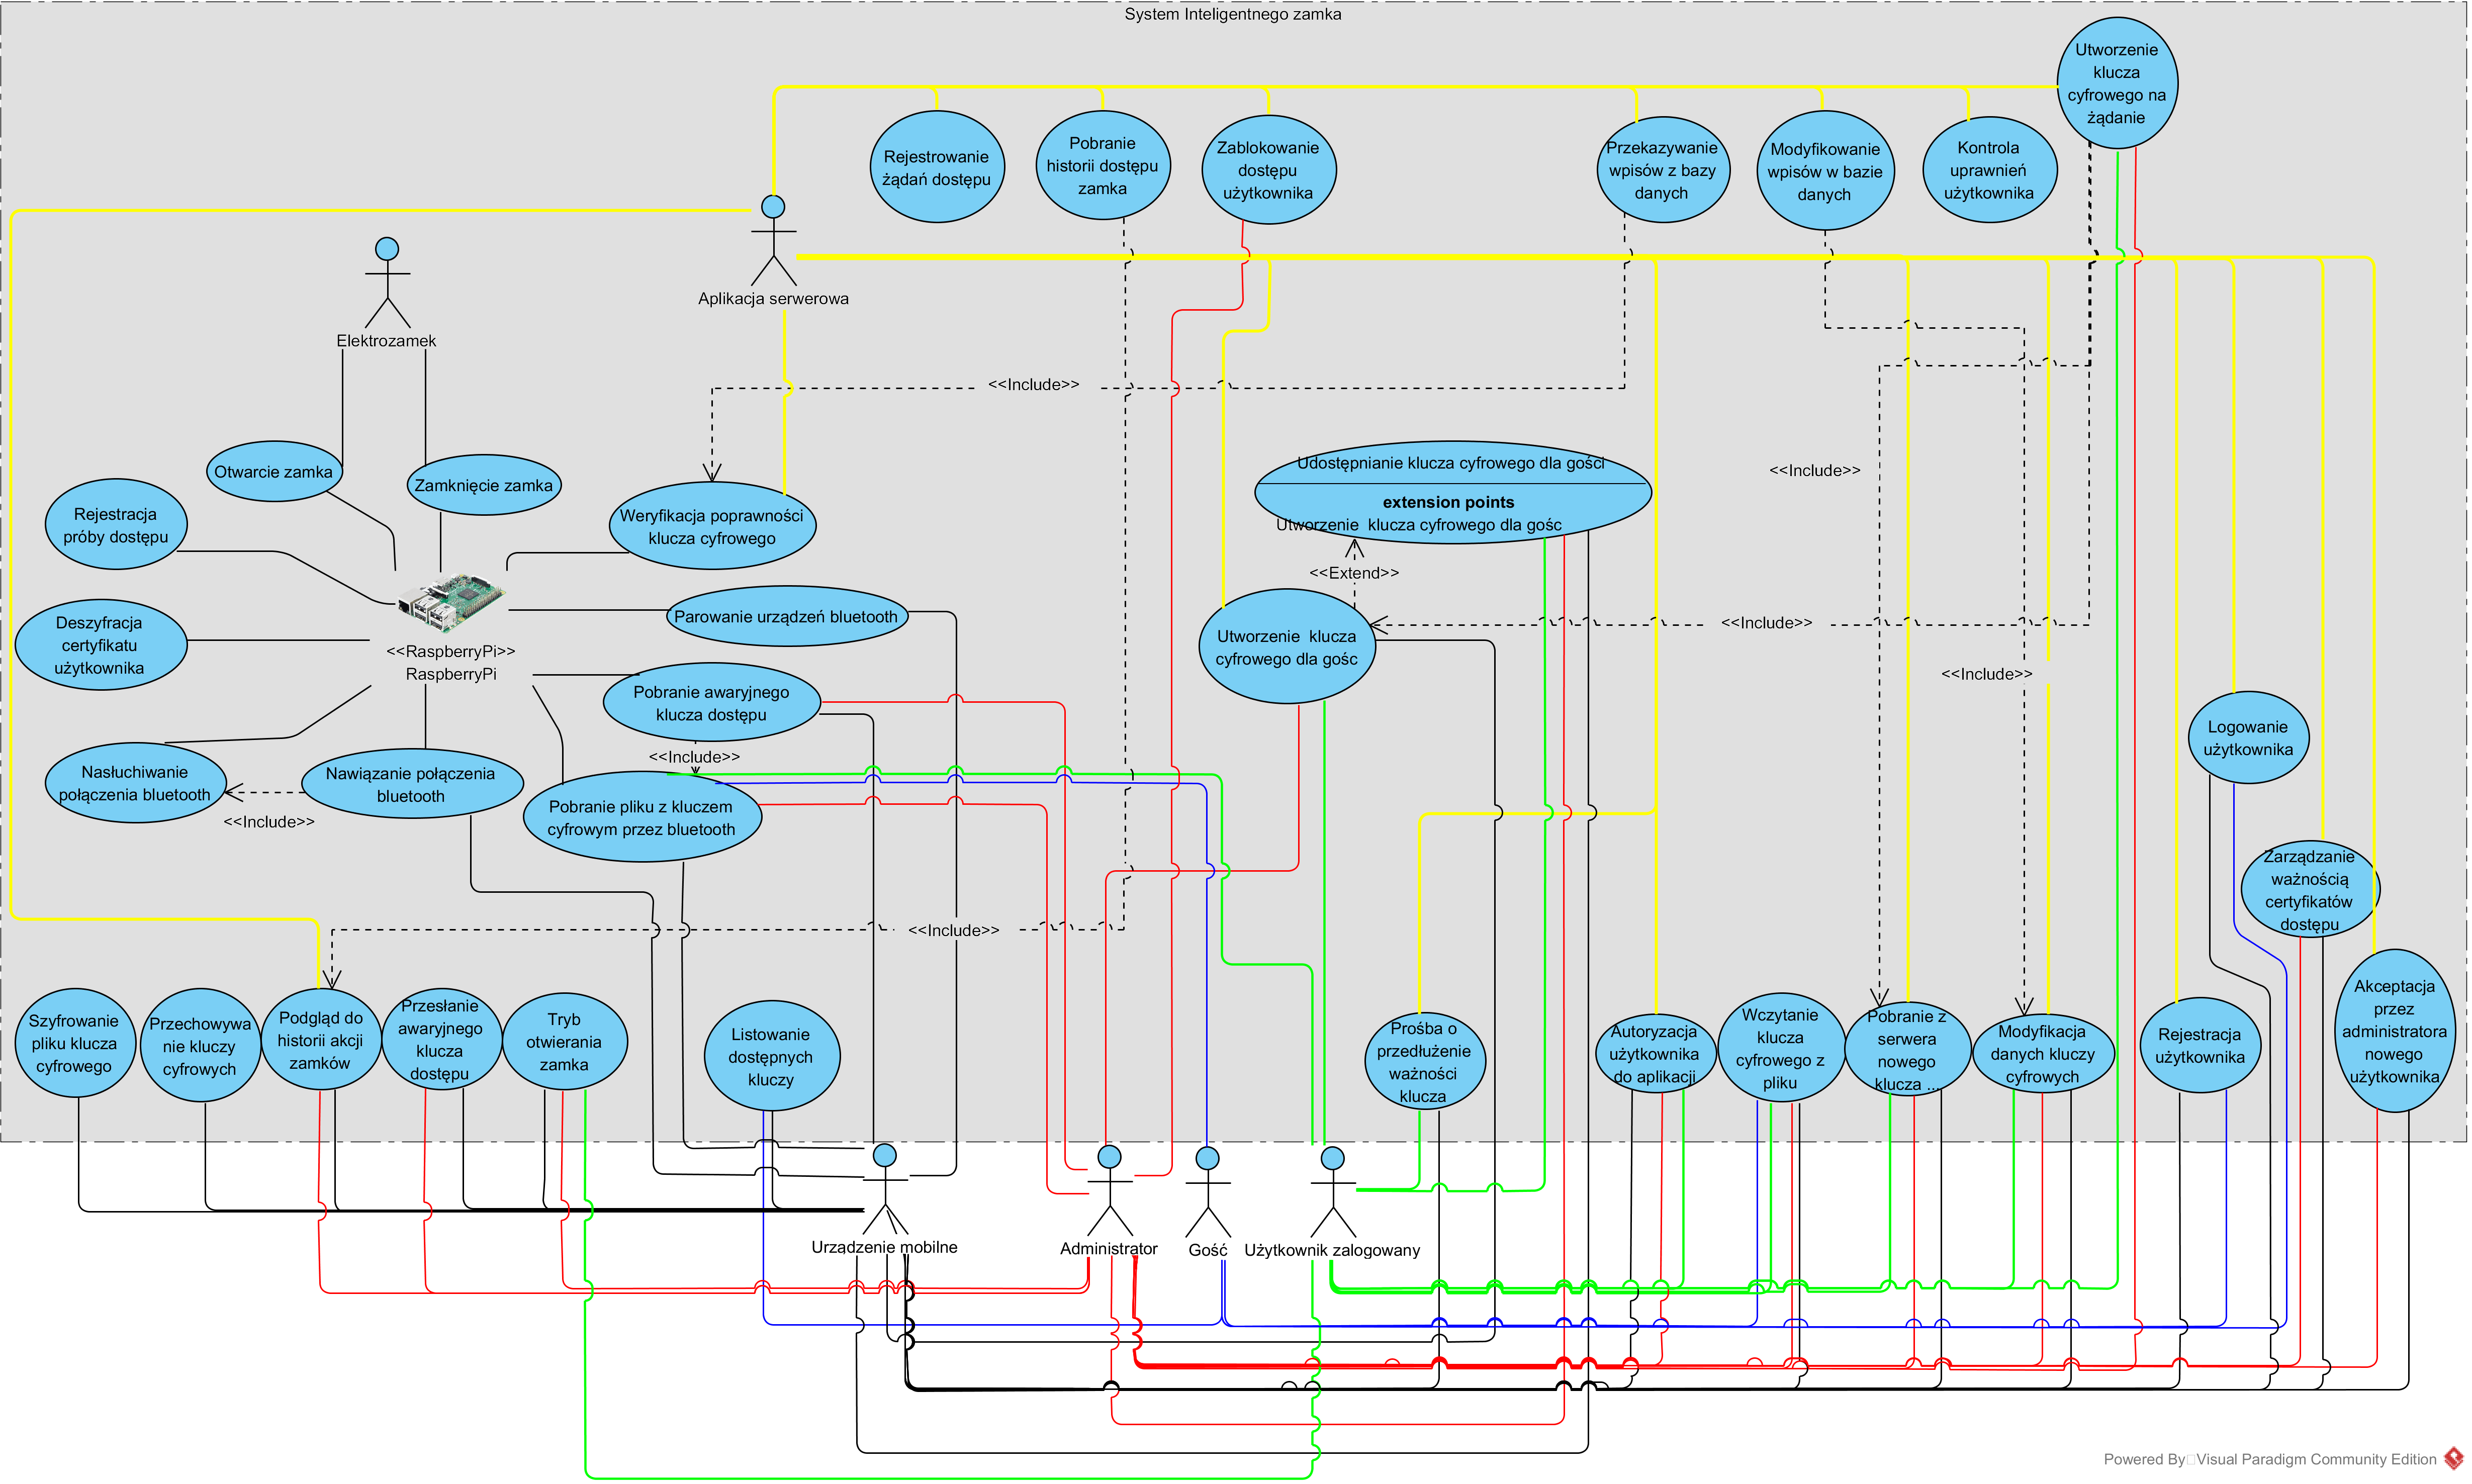
\includegraphics[width=24cm]{Obrazy/Diagram_przypadkow_uzycia.png}
			\caption{Diagram przypadków użycia}
			\label{diagram:diagram przypadków_użycia}
		\end{figure}
	\end{landscape}
\newpage
	\subsubsection[Projekt bazy danych]{Projekt bazy danych [Maciej Marciniak]} 
	Baza danych będzie składać się z pięciu tabel:
	\begin{itemize*}
		\item {USERS} --- przechowuje dane użytkowników oraz dane niezbędne przy weryfikacji logowania,
		\item {LOCKS} --- zawiera informacje na temat dostępnych w systemie zamków,
		\item {ACCESS\_TO\_LOCKS} --- archiwizuje próby użycia certyfikatów,
		\item {LOCKS\_KEYS} --- zawiera wszystkie klucze dostępowe użytkowników,
		\item {WAIT\_LOCKS\_KEYS} --- przetrzymuje klucze dostępowe oczekujące na zatwierdzenie przez administratora.
	\end{itemize*}
	
	Wiersz tabeli USERS zawierać musi:
	\begin{itemize*}
		\item {ID\_USER} --- unikalny identyfikator (klucz główny) użytkownika składający się z 10 cyfr,
		\item {LOGIN} --- unikalna nazwa użytkownika niezbędna podczas logowania, zawierająca nie więcej niż 255 znaków,
		\item {PASSWORD} --- hasło zapisane w postaci skrótu, potrzebne do autoryzacji dostępu użytkownikowi,
		\item {NAME} - imię użytkownika,
		\item {SURNAME} --- nazwisko użytkownika,
		\item {TOKEN} --- generowany ciąg pseudolosowy klucz sesji logowania,
		\item  {ISACTIVATED} --- pole boolowskie oznaczające, czy dane konto jest zaakceptowane,
		\item {IS\_ADMIN} --- pole boolowskie wskazujące czy dany użytkownik jest administratorem czy nie, (aktywowane) przez administratora.
		\item {PUBLIC\_KEY} --- klucz publiczny użytkownika potrzebny do podpisu cyfrowego,
		\item Serial\_number --- unikalny numer seryjny certyfikatu szyfrującego,
		\item Validity\_period --- data do której ważny jest certyfikat szyfrujący,
		\item Version --- numer wersji certyfikatu szyfrującego,
		\item Signature\_Algorithm\_Identifier --- identyfikator algorytmu szyfrującego,
		\item Hash\_Algorithm --- identyfikator algorytmu funkcji skrótu.
	\end{itemize*}
	
	Klucz dostępowy składa się z:
	\begin{itemize*}
		\item {ID\_KEY} --- unikalny identyfikator (klucz główny) klucza dostępowego składający się z 10 cyfr,
		\item {ID\_LOCK} --- klucz obcy do tabeli przechowującej dostępne zamki,
		\item {ID\_USER} --- klucz obcy do tabeli przechowującej dane użytkownika, jest to pole służące do określenia kto utworzył klucz dostępu,
		\item {LOCK\_KEY} --- unikalna wartość certyfikatu dostępu,
		\item {FROM\_DATE} --- data od której obowiązuje klucz,
		\item {TO\_DATE} --- data do której obowiązuje klucz,
		\item {ISACTUAL} --- data wygaśnięcia klucza, jeśli równa TO, oznacza to że klucz utracił ważność z powodu czasu, jeśli różna oznacza, to że zablokowano z innego powodu ważność,
		\item {MONDAY} --- słowne określenie, w których godzinach zostanie przyznany dostęp w poniedziałki,
		\item {TUESDAY} --- słowne określenie, w których godzinach zostanie przyznany dostęp we wtorki,
		\item {WEDNESDAY} --- słowne określenie, w których godzinach zostanie przyznany dostęp w środy,
		\item {THURSDAY} --- słowne określenie, w których godzinach zostanie przyznany dostęp w czwartki,
		\item {FRIDAY} --- słowne określenie, w których godzinach zostanie przyznany dostęp w piątki,
		\item {SATURDAY} --- słowne określenie, w których godzinach zostanie przyznany dostęp w soboty,
		\item {SUNDAY} --- słowne określenie, w których godzinach zostanie przyznany dostęp w niedziele,
		\item {IS\_PERNAMENT} --- zmienna boolowska oznaczająca czy dostęp jest zawsze,
		\item {NAME} - imię osoby, której dotyczy certyfikat,
		\item {SURNAME} --- nazwisko osoby, której dotyczy certyfikat.
	\end{itemize*}

\newpage
	Zamek opisywany jest poprzez kolumny:
	\begin{itemize*}
		\item {ID\_LOCK} --- unikalny identyfikator (klucz główny) zamka składający się z 10 cyfr,
		\item {NAME} --- unikalna nazwa zamka,
		\item {MAC\_ADDRESS} --- adres fizyczny urządzenia sterującego zamkiem,
		\item {LOCALIZATION} --- nieobowiązkowe pole opisujące fizyczne położenie zamka,
		\item {People\_inside} --- wartość licznika osób znajdujących się wewnątrz pomieszczenia.
	\end{itemize*}

	W tabeli archiwizującej akcje na zamku znajdują się takie dane jak:
	\begin{itemize*}
		\item {ID} --- unikalny identyfikator (klucz główny) akcji wykonanej na certyfikacie składający się z 10 cyfr,
		\item {ID\_KEY} --- klucz obcy do tabeli przechowującej klucze dostępowe, dzięki tej informacji możemy uzyskać dane o zamku, który został otwierany jak również do kogo należał klucz,
		\item {DATE} --- dokładna data z godziną użycia klucza dostępowego,
		\item {ACCESS} --- binarna flaga informująca czy dostęp został przyznany czy odmówiony.
	\end{itemize*}

	Tabela WAIT\_LOCKS\_KEYS składa się z:
	\begin{itemize*}
		\item {ID\_KEY} --- unikalny identyfikator (klucz główny) oczekującego certyfikatu,
		\item{ID\_LOCK} --- klucz obcy do tabeli LOCKS, oznacza zamek do którego jest zgłaszana prośba dostępu,
		\item {ID\_USER} --- klucz obcy do tabeli USERS, oznacza użytkownika który zgłasza prośbę o dostęp do zamka.
	\end{itemize*}
	
	Diagramy bazy danych odpowiednio encji i relacji przedstawione zostały na Rys \ref{diagram:diagram encji} i Rys. \ref{diagram:diagram relacji}.\cite{BD}  
	
	\begin{figure}[!h]
		\centering
		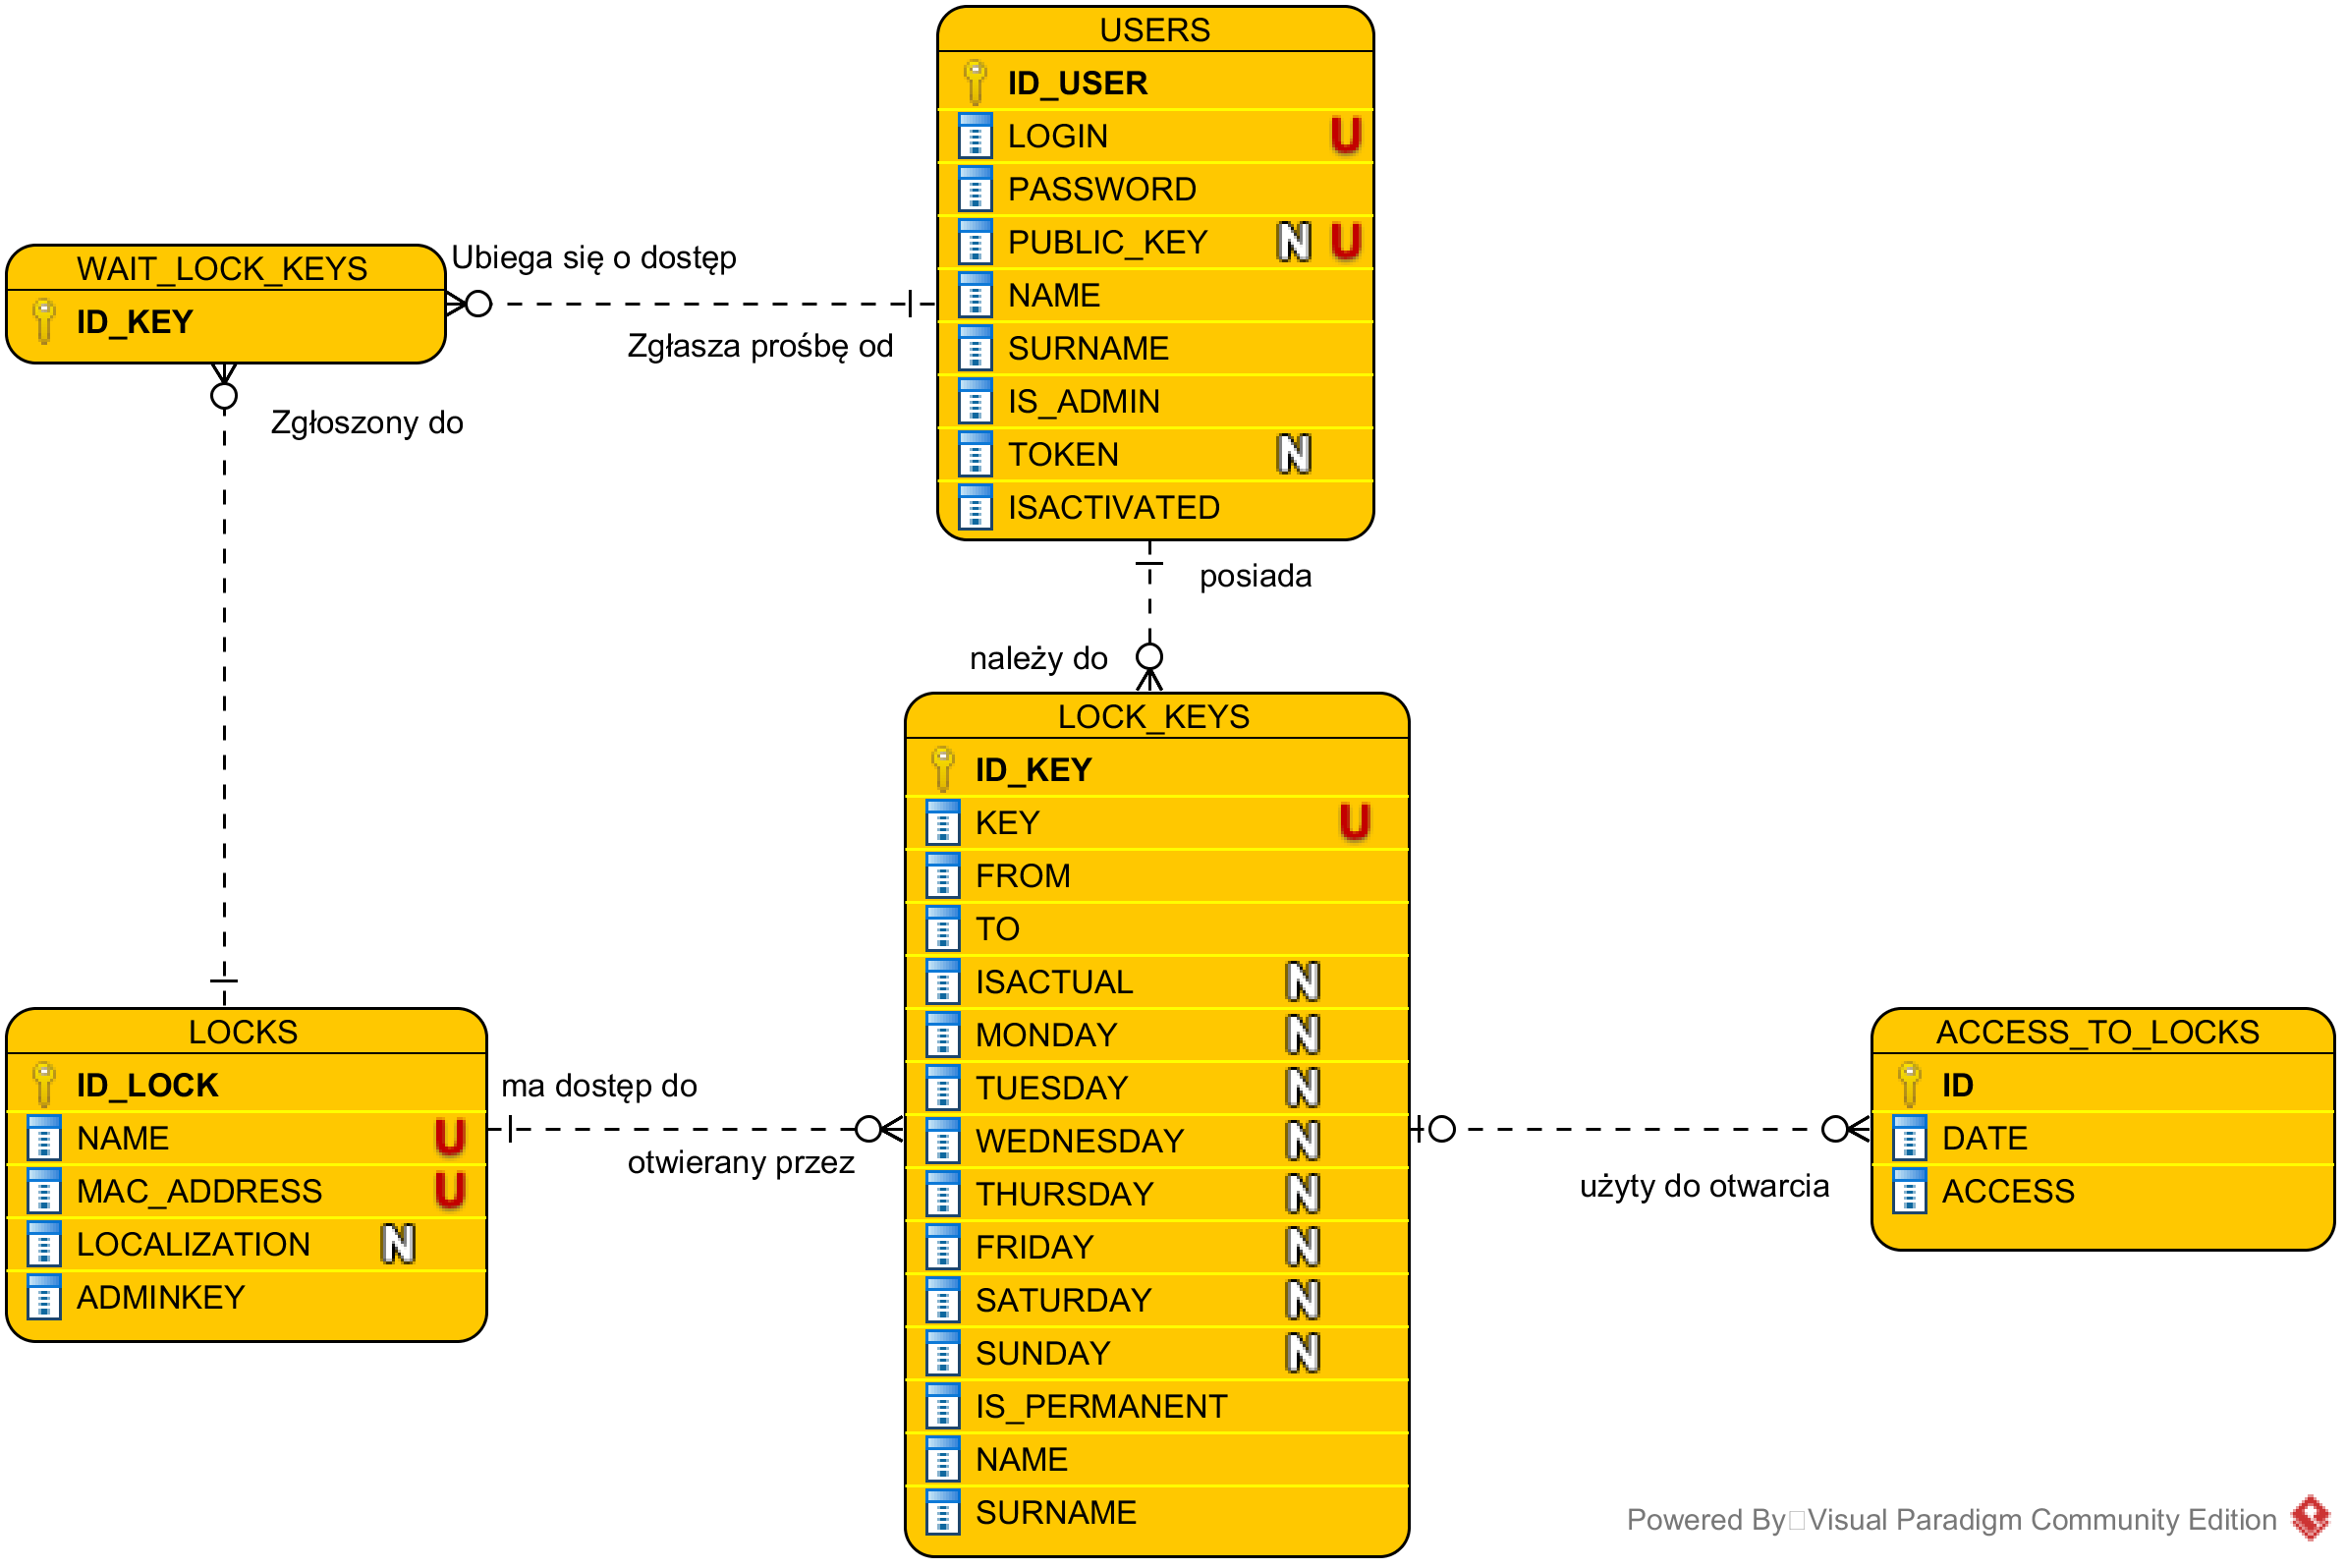
\includegraphics[width=13cm]{Obrazy/Diagram_encji.png}
		\caption{Diagram encji bazy danych}
		\label{diagram:diagram encji}
	\end{figure}
	\newpage
	\begin{figure}[!h]
		\centering
		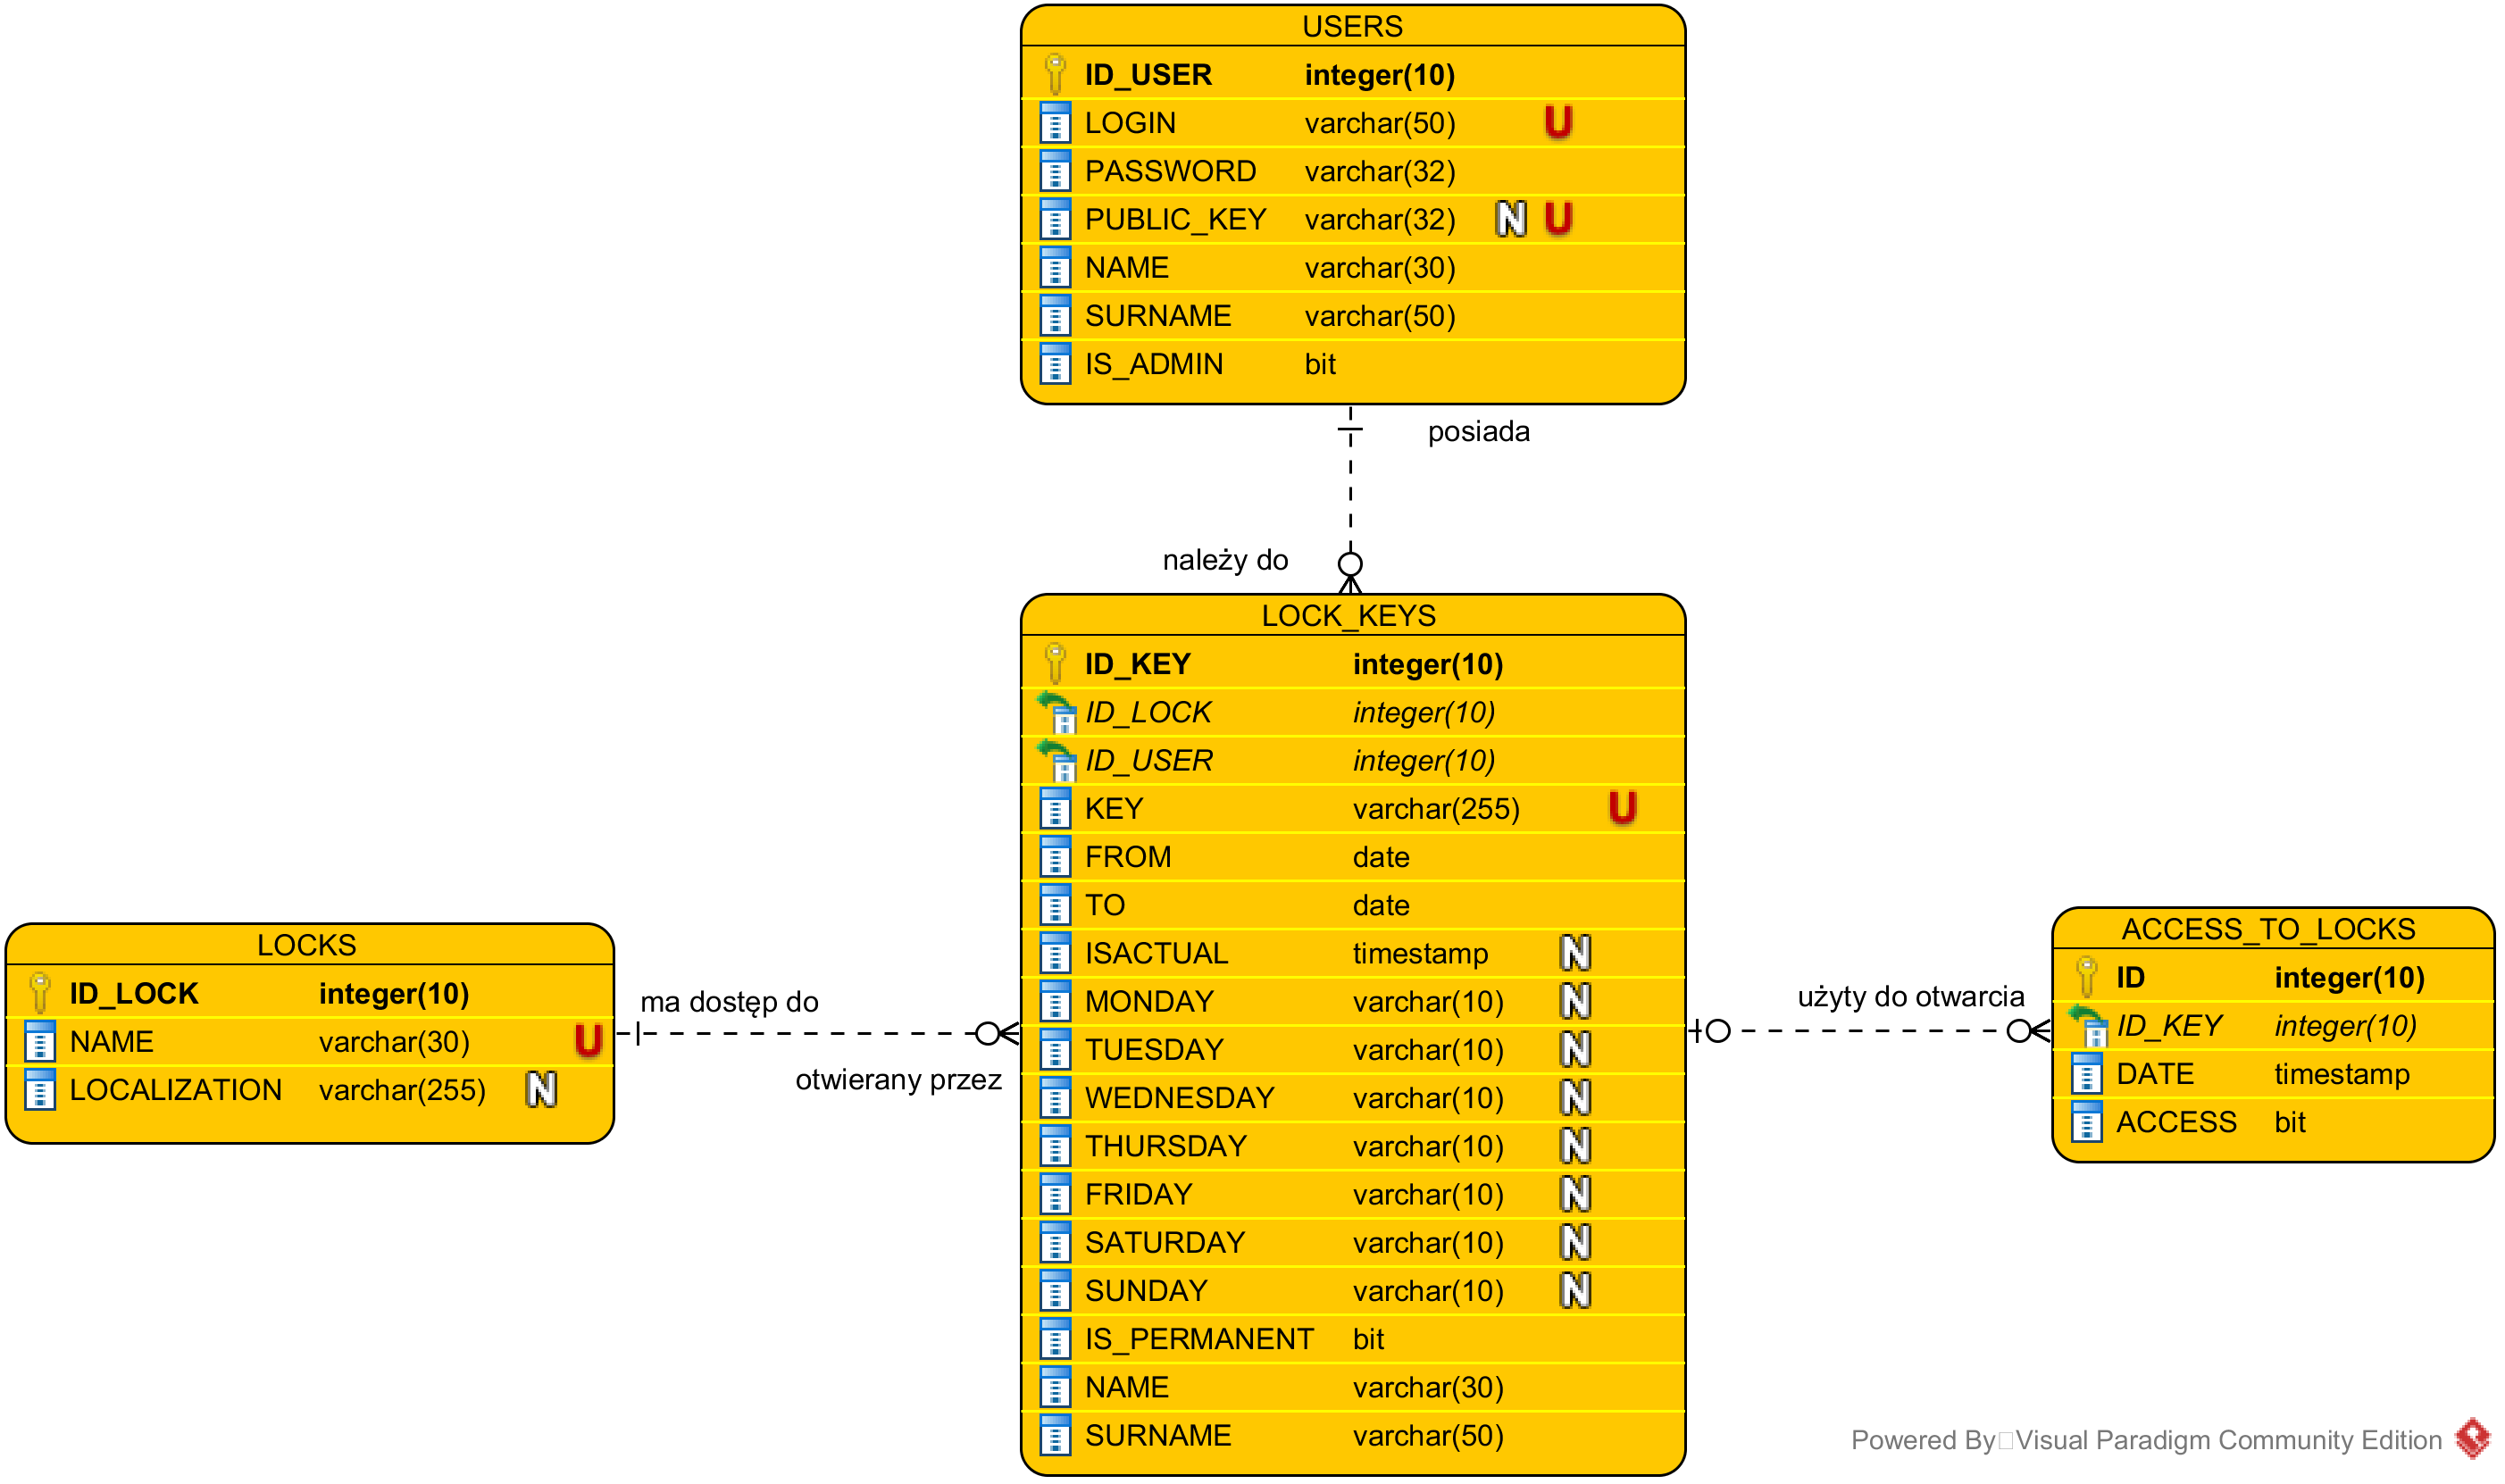
\includegraphics[width=13cm]{Obrazy/Diagram_relacji.png}
		\caption{Diagram relacji bazy danych}
		\label{diagram:diagram relacji}
	\end{figure}
\newpage

	\subsubsection{Diagramy klas}
		\paragraph{Aplikacja mobilna [Damian Filipowicz]}
		Aplikacja mobilna składa się z szeregu klas napisanych w 2 językach: Kotlin oraz Java. Ponadto klasy te zostały podzielone na 5 kategorii (Rys. \ref{Schemat ogólny diagramu klas dla Aplikacji mobilnej}) takich jak:
		\begin{itemize*}
			\item API 
			(Rys. \ref{Diagram klas dla paczki api}) 
			---  które przechowuje klasy odpowiedzialne za funkcje wykorzystywane w wielu miejscach systemu. W paczce znajdują się klasy odpowiedzialne między innymi za odczyt oraz zapis do pliku, komunikacje HTTPS, czy wykorzystywanie SharedPreferences w aplikacji ,
			\item Navigation 
			(Rys. \ref{Diagram klas dla paczki navigations}) 
			--- są to klasy odpowiedzialne za generowanie nawigacji w aplikacji mobilnej. Paczka znajdują się 4 klasy,
			\item Adapters
			(Rys. \ref{Diagram klas dla paczki adapters}) 
			 --- w którym są przechowywane klasy adapter wykorzystywane w systemie do wyświetlania danych,
		\end{itemize*}
	
	\begin{figure}[ht!]
		\centering
		\vspace{-0.6cm}
		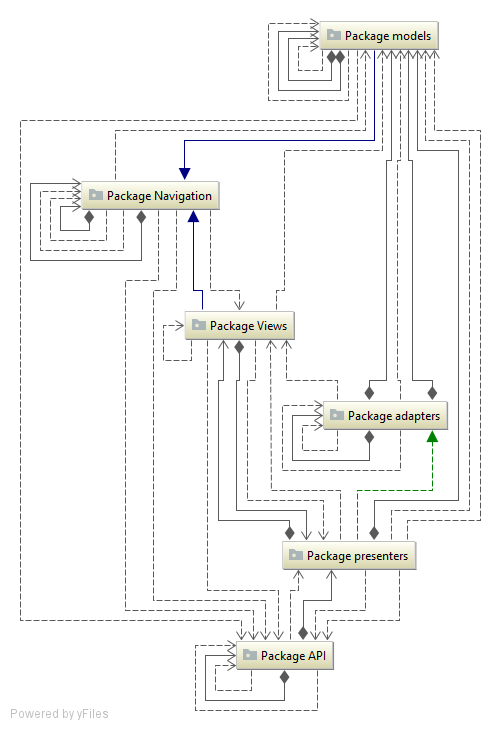
\includegraphics[width=11cm]{Obrazy/AM_DK_ALL}
		\caption{Schemat ogólny diagramu klas dla Aplikacji Mobilnej}
		\label{Schemat ogólny diagramu klas dla Aplikacji mobilnej}
	\end{figure}
	\newpage
\begin{figure}[ht!]
	\centering
	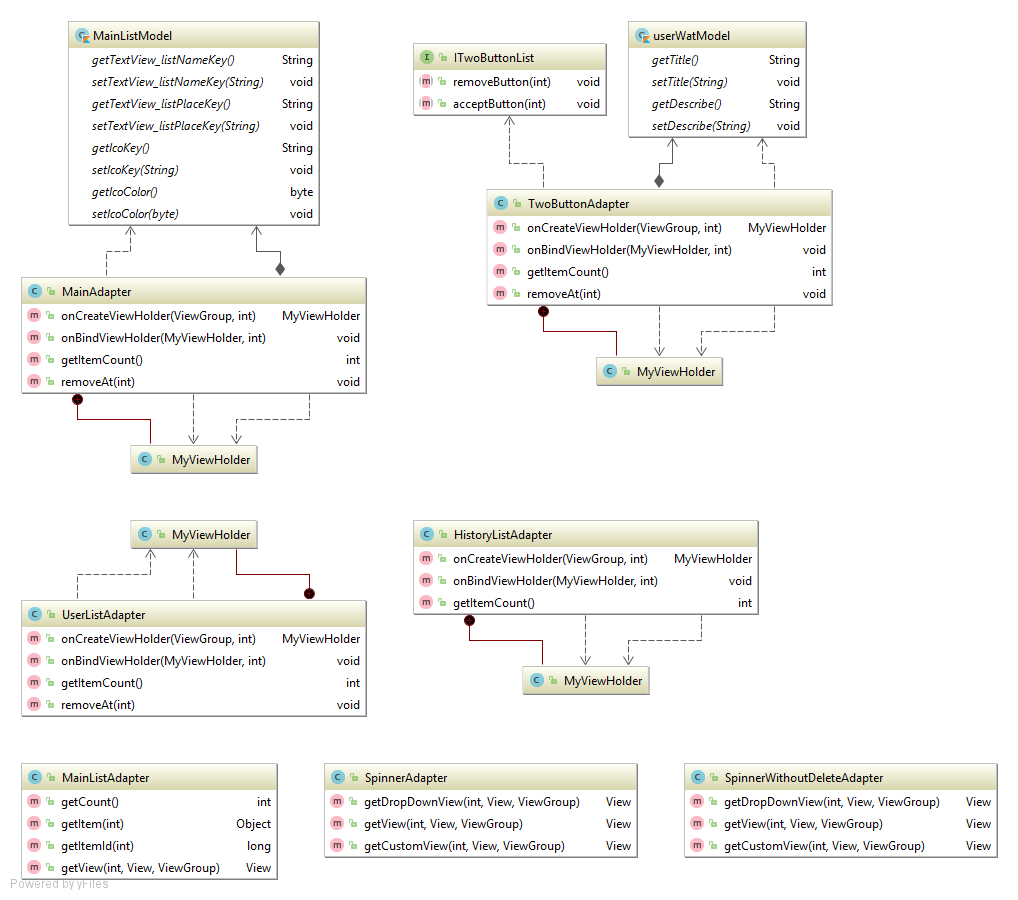
\includegraphics[width=16cm]{Obrazy/AM_DK_adapter}
	\caption{Diagram klas dla paczki adapters}
	\label{Diagram klas dla paczki adapters}
\end{figure}
\newpage
\begin{figure}[ht!]
	\centering
	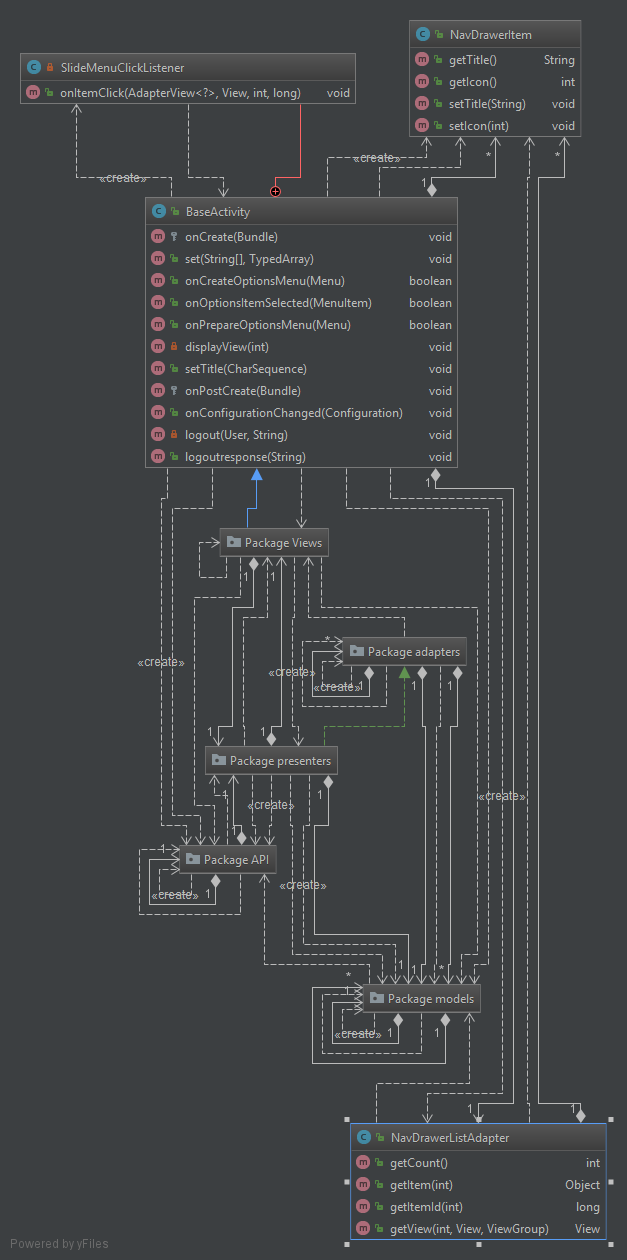
\includegraphics[width=16cm]{Obrazy/AM_DK_navigation}
	\caption{Diagram klas dla paczki navigations}
	\label{Diagram klas dla paczki navigations}
\end{figure}

Oprócz tych wymienionych wyżej są dodatkowo 3 kategorie implementujące wzorzec architektoniczny Model-View-Presenter i są to odpowiednio:
\begin{itemize*}
\item Model (Rys. \ref{Diagram klas dla paczki models}) 
--- przechowujący klasy modele odpowiedzialne za przechowywanie danych. Każda z klas która jest powiązana z odpowiednim widokiem   w nazwie na początku ma nazwę widoku a na końcu ma słowo Model,   
\item View 
(Rys. \ref{Diagram klas dla paczki views}) 
--- przechorowujący klasy widoków odpowiedzialne za generowanie widoków w aplikacji. Każda z klas która jest powiązana z odpowiednim widokiem   w nazwie na początku ma nazwę widoku a na końcu ma słowo Activity, 
\item Presenter
(rysunek \ref{Diagram klas dla paczki presenters}) 
--- przechowujący klasy presenter odpowiedzialne za interakcje pomiędzy modelami oraz widokami. Każda z klas, która jest powiązana z odpowiednim widokiem w nazwie na początku ma nazwę widoku, a na końcu ma słowo Presenter.\cite{And}
\end{itemize*}
\newpage
\begin{figure}[ht!]
	\centering
	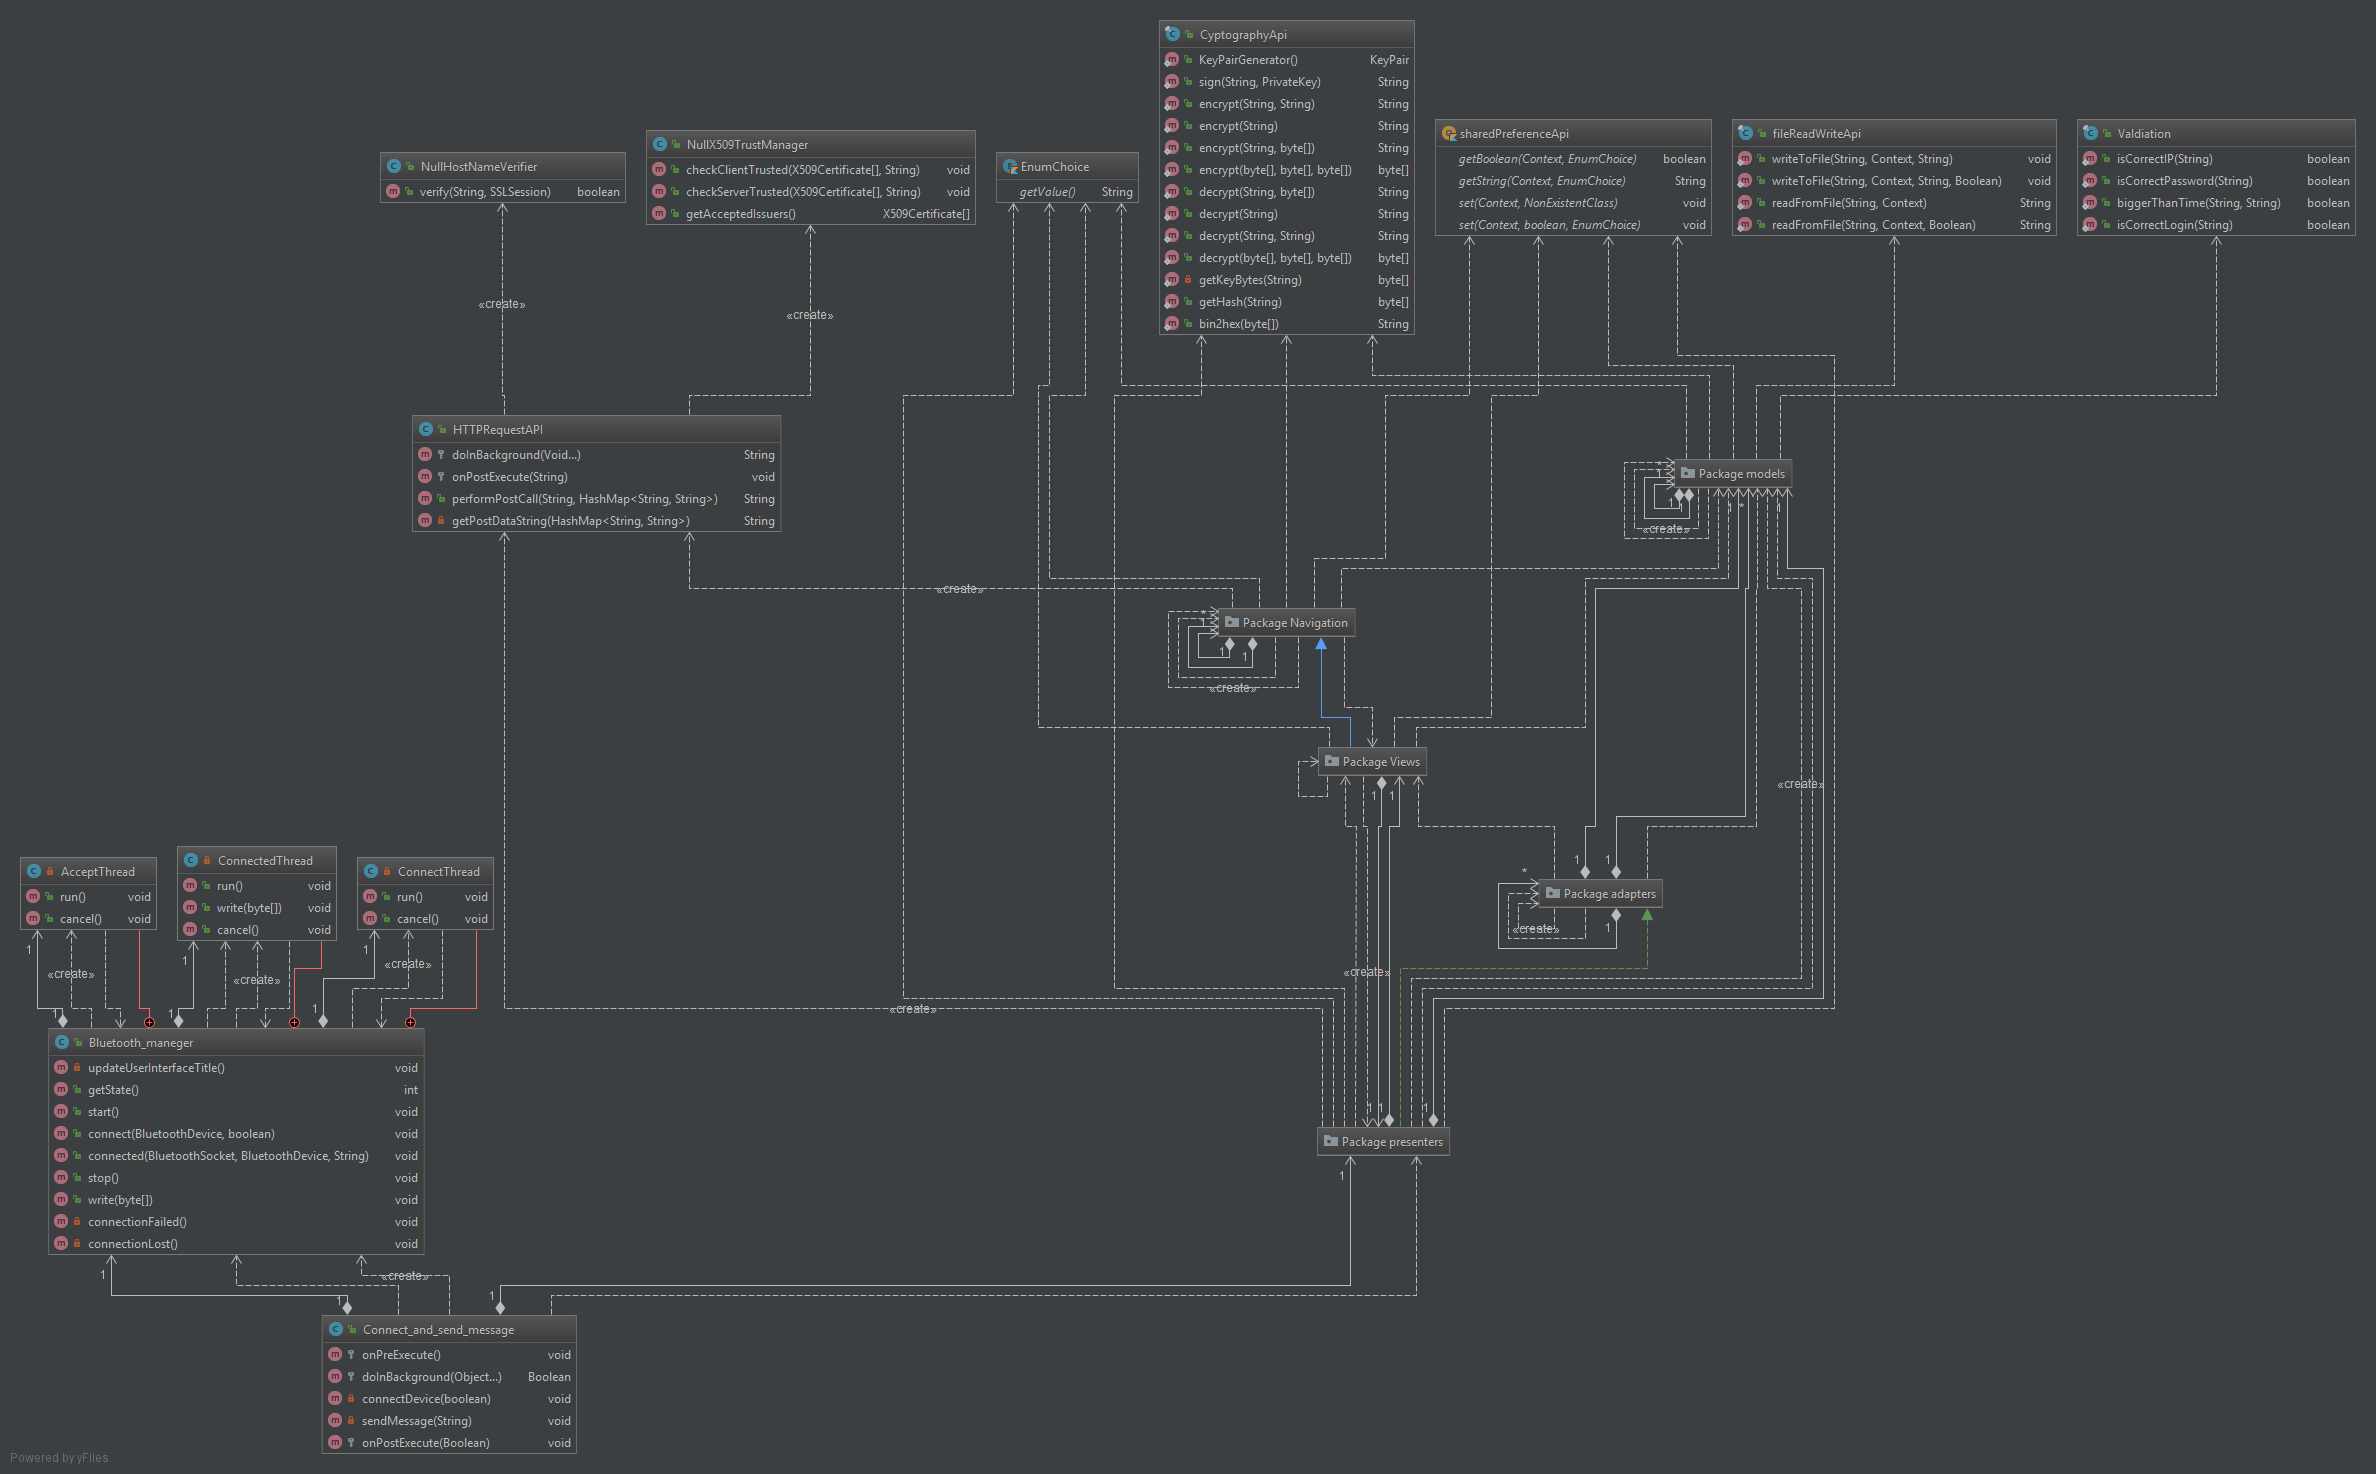
\includegraphics[width=15cm]{Obrazy/AM_DK_api}
	\caption{Diagram klas dla paczki api}
	\label{Diagram klas dla paczki api}
\end{figure}
\newpage

		\newpage
	\begin{figure}[ht!]
		\centering
		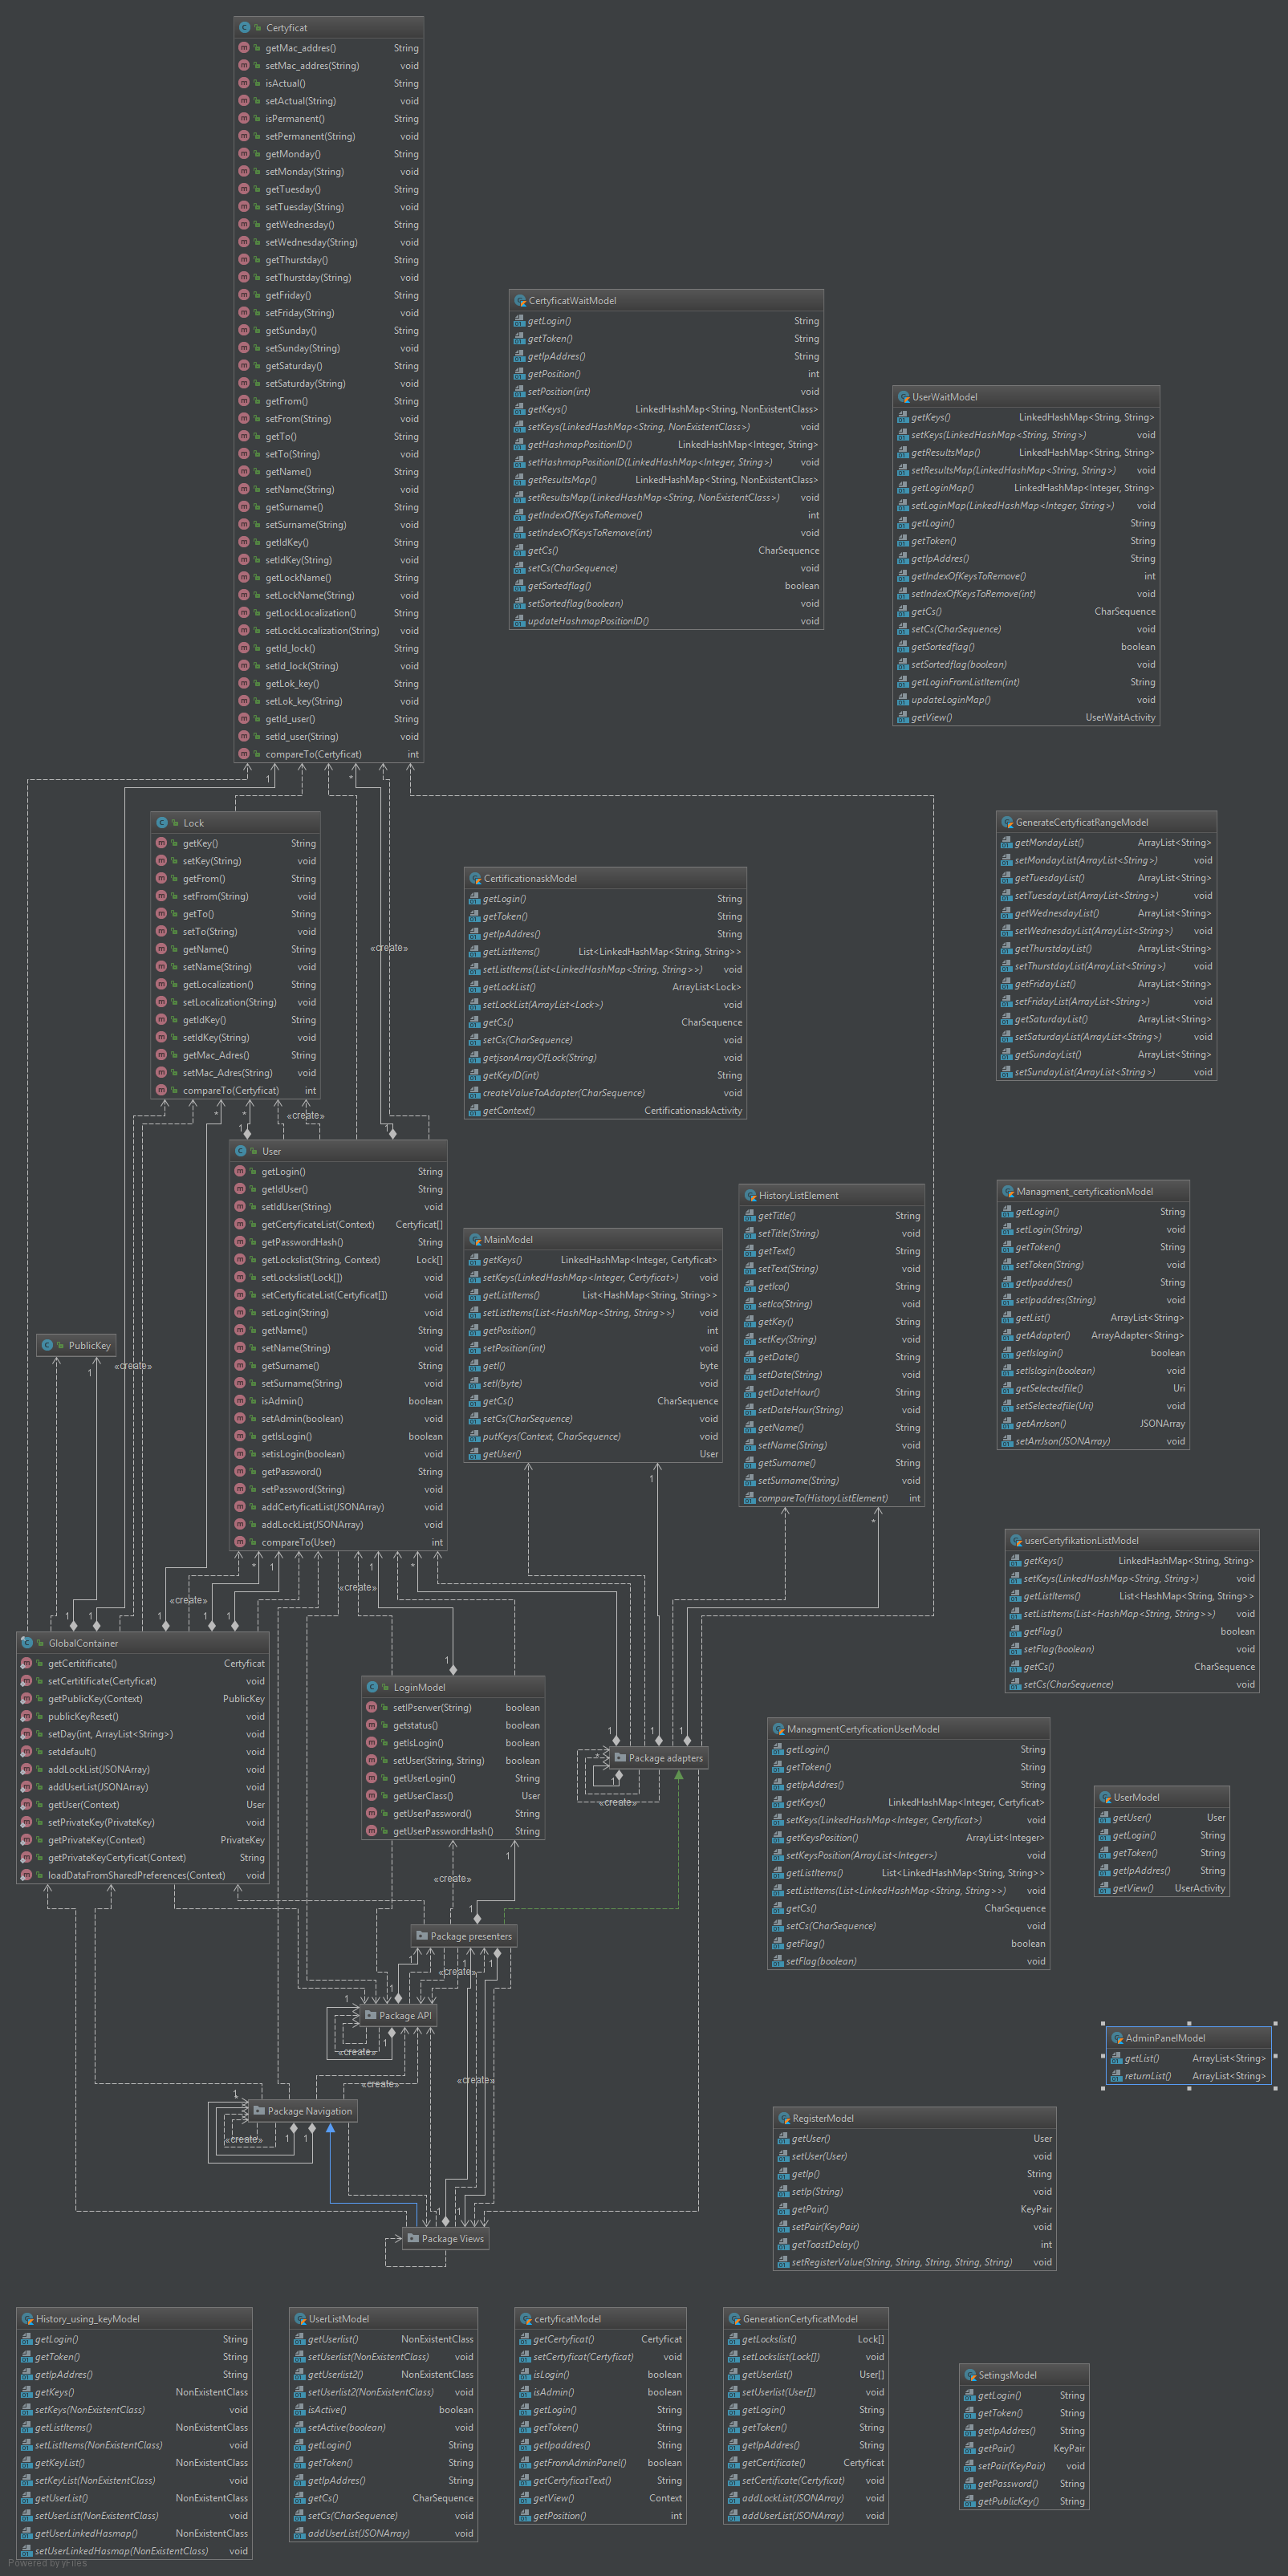
\includegraphics[width=16cm]{Obrazy/AM_DK_model}
		\caption{Diagram klas dla paczki models}
		\label{Diagram klas dla paczki models}
	\end{figure}

	\newpage
\begin{figure}[ht!]
	\centering
	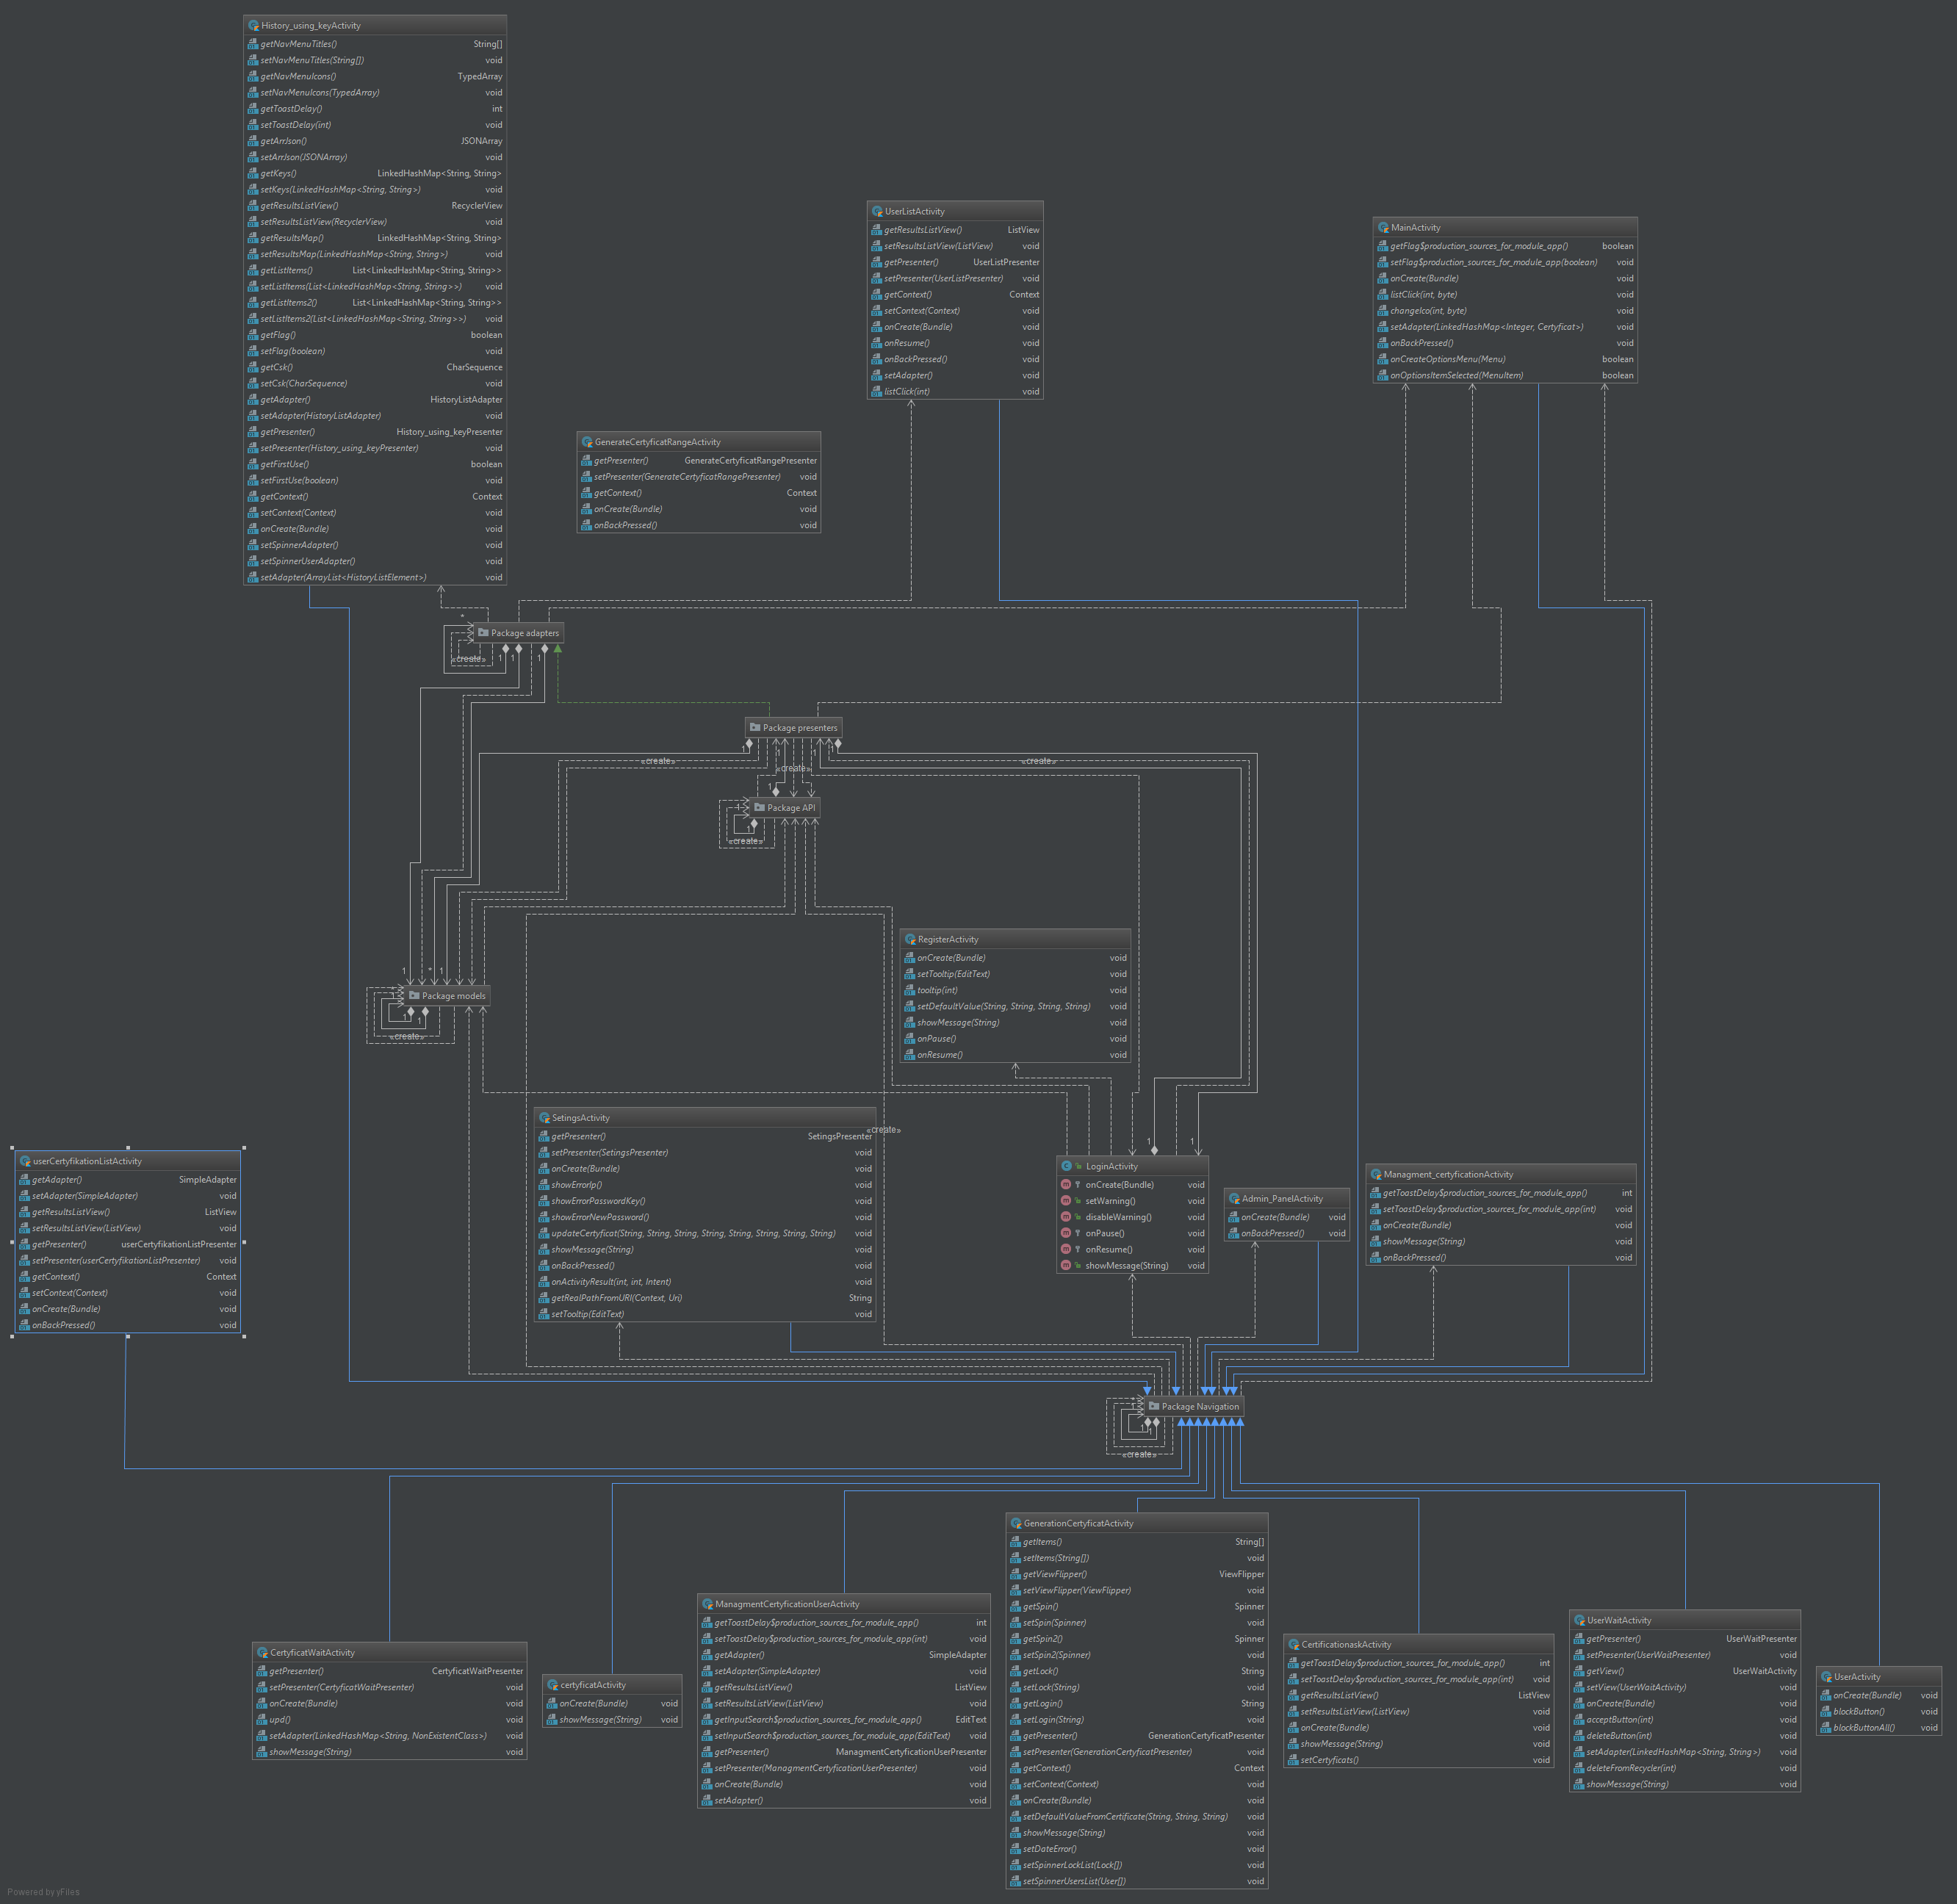
\includegraphics[width=16cm]{Obrazy/AM_DK_view}
	\caption{Diagram klas dla paczki views}
	\label{Diagram klas dla paczki views}
\end{figure}
\newpage

		\begin{figure}[ht!]
			\centering
			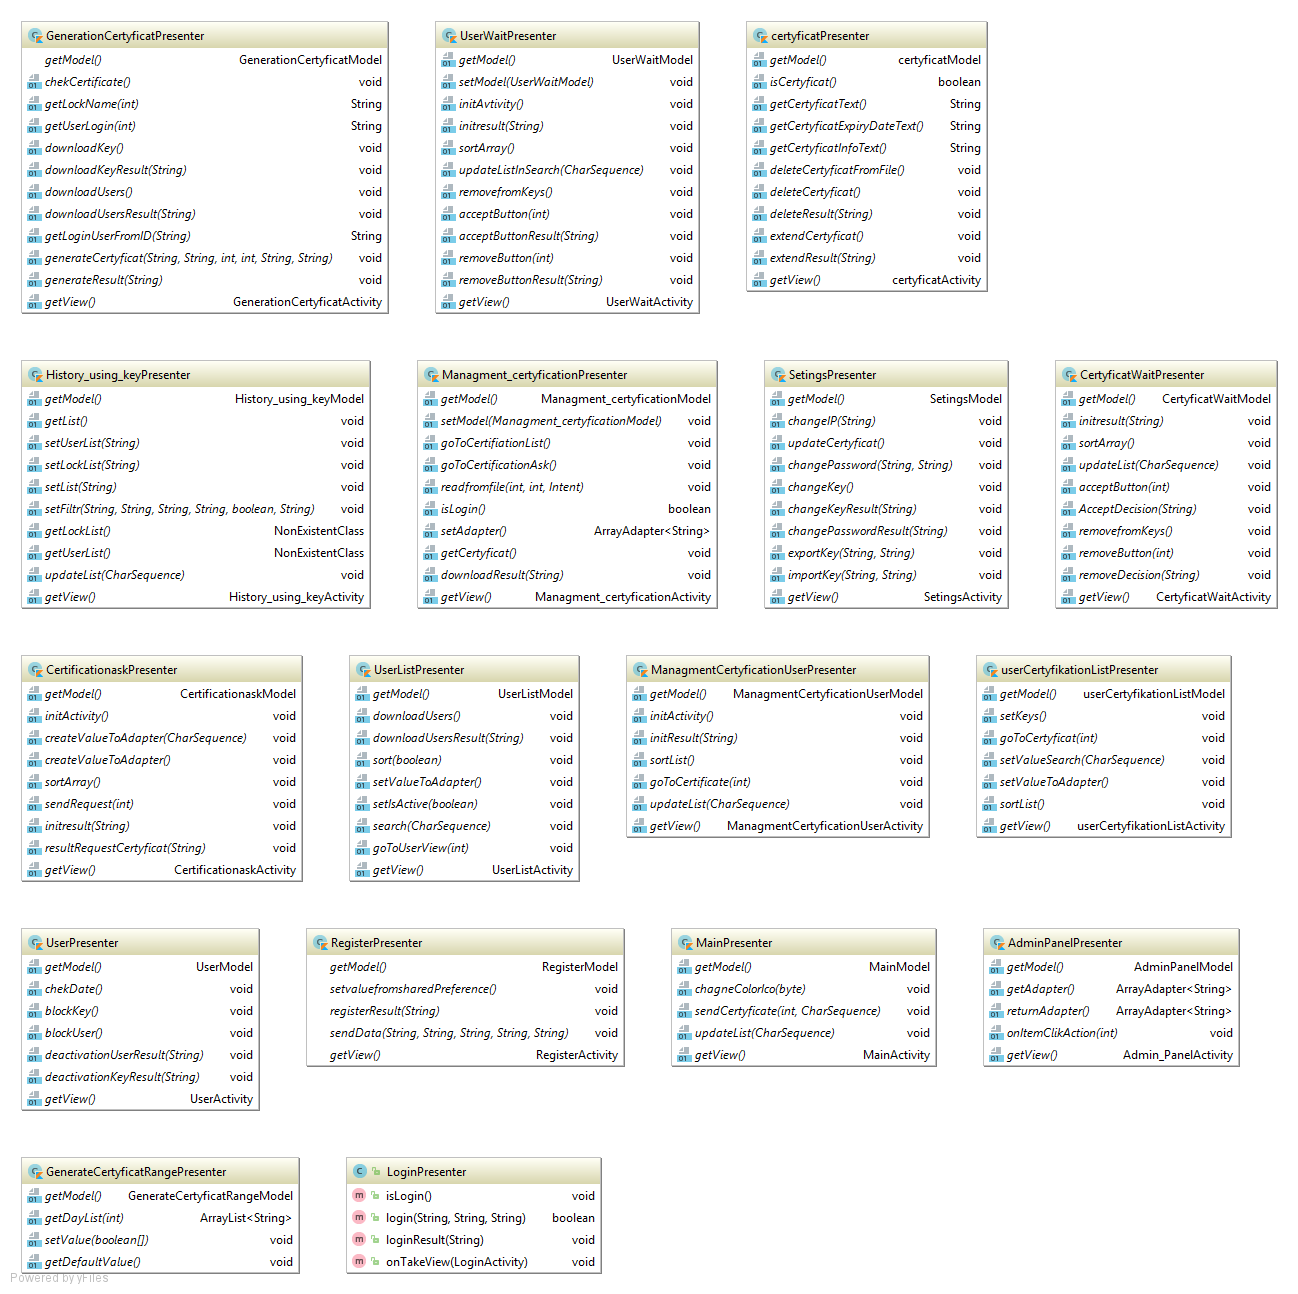
\includegraphics[width=16cm]{Obrazy/AM_DK_presenter}
			\caption{Diagram klas dla paczki presenters}
			\label{Diagram klas dla paczki presenters}
		\end{figure}
		\newpage		

	\paragraph{Aplikacja serwera [Maciej Marciniak]}
	Diagram klas znajdujący się na Rys. \ref{diagram:Diagram_klas_aplikacji_serwerowej} przedstawia klasy i metody potrzebne do realizacji projektu. Klasa Views przechowuje funkcje wykonujące akcje na bazie danych, zaś klasa URLs odpowiada za wskazanie pod jakim adresem URL znajduje się konkretna funkcja. Nazwy oraz budowę klas narzuca framework Django. Każda nazwa funkcji odpowiada nazwie URLa oraz opisuje jaką funkcję ma pełnić.
	
	\paragraph{Urządzenie sterujące [Maciej Marciniak]}
	Zaprojektowane klasy, które mają zostać zaimplementowane w urządzeniu sterującym znajdują się na Rys. \ref{diagram:Diagram_klas_urzadzenia_sterujacego}. Klasa Main jest głównym elementem programu. W niej wywołana ma zostać funkcja ''main'' (język Python nie wymaga funkcji niesocjalizującej charakterystycznej dla innych języków programowania). Obiekty klasy Certificate i CertificatePKI odpowiednio przechowywać mają dane certyfikatów dostępowych i szyfrujących. Metoda w Main Compare\_PKI\_Certificate porównywać ma klucze szyfrujące, czy są identyczne. Klasa Servo zarządzać ma fizycznym zamkiem przy drzwiach, uniwersalnie dla serwomechanizmu oraz elektrozamka. Funkcja Open ma mieć na celu ustawienie zamka w stanie otwartym, zaś Close analogicznie zamkniętym. 
	
	\begin{figure}[!h]
		\centering
		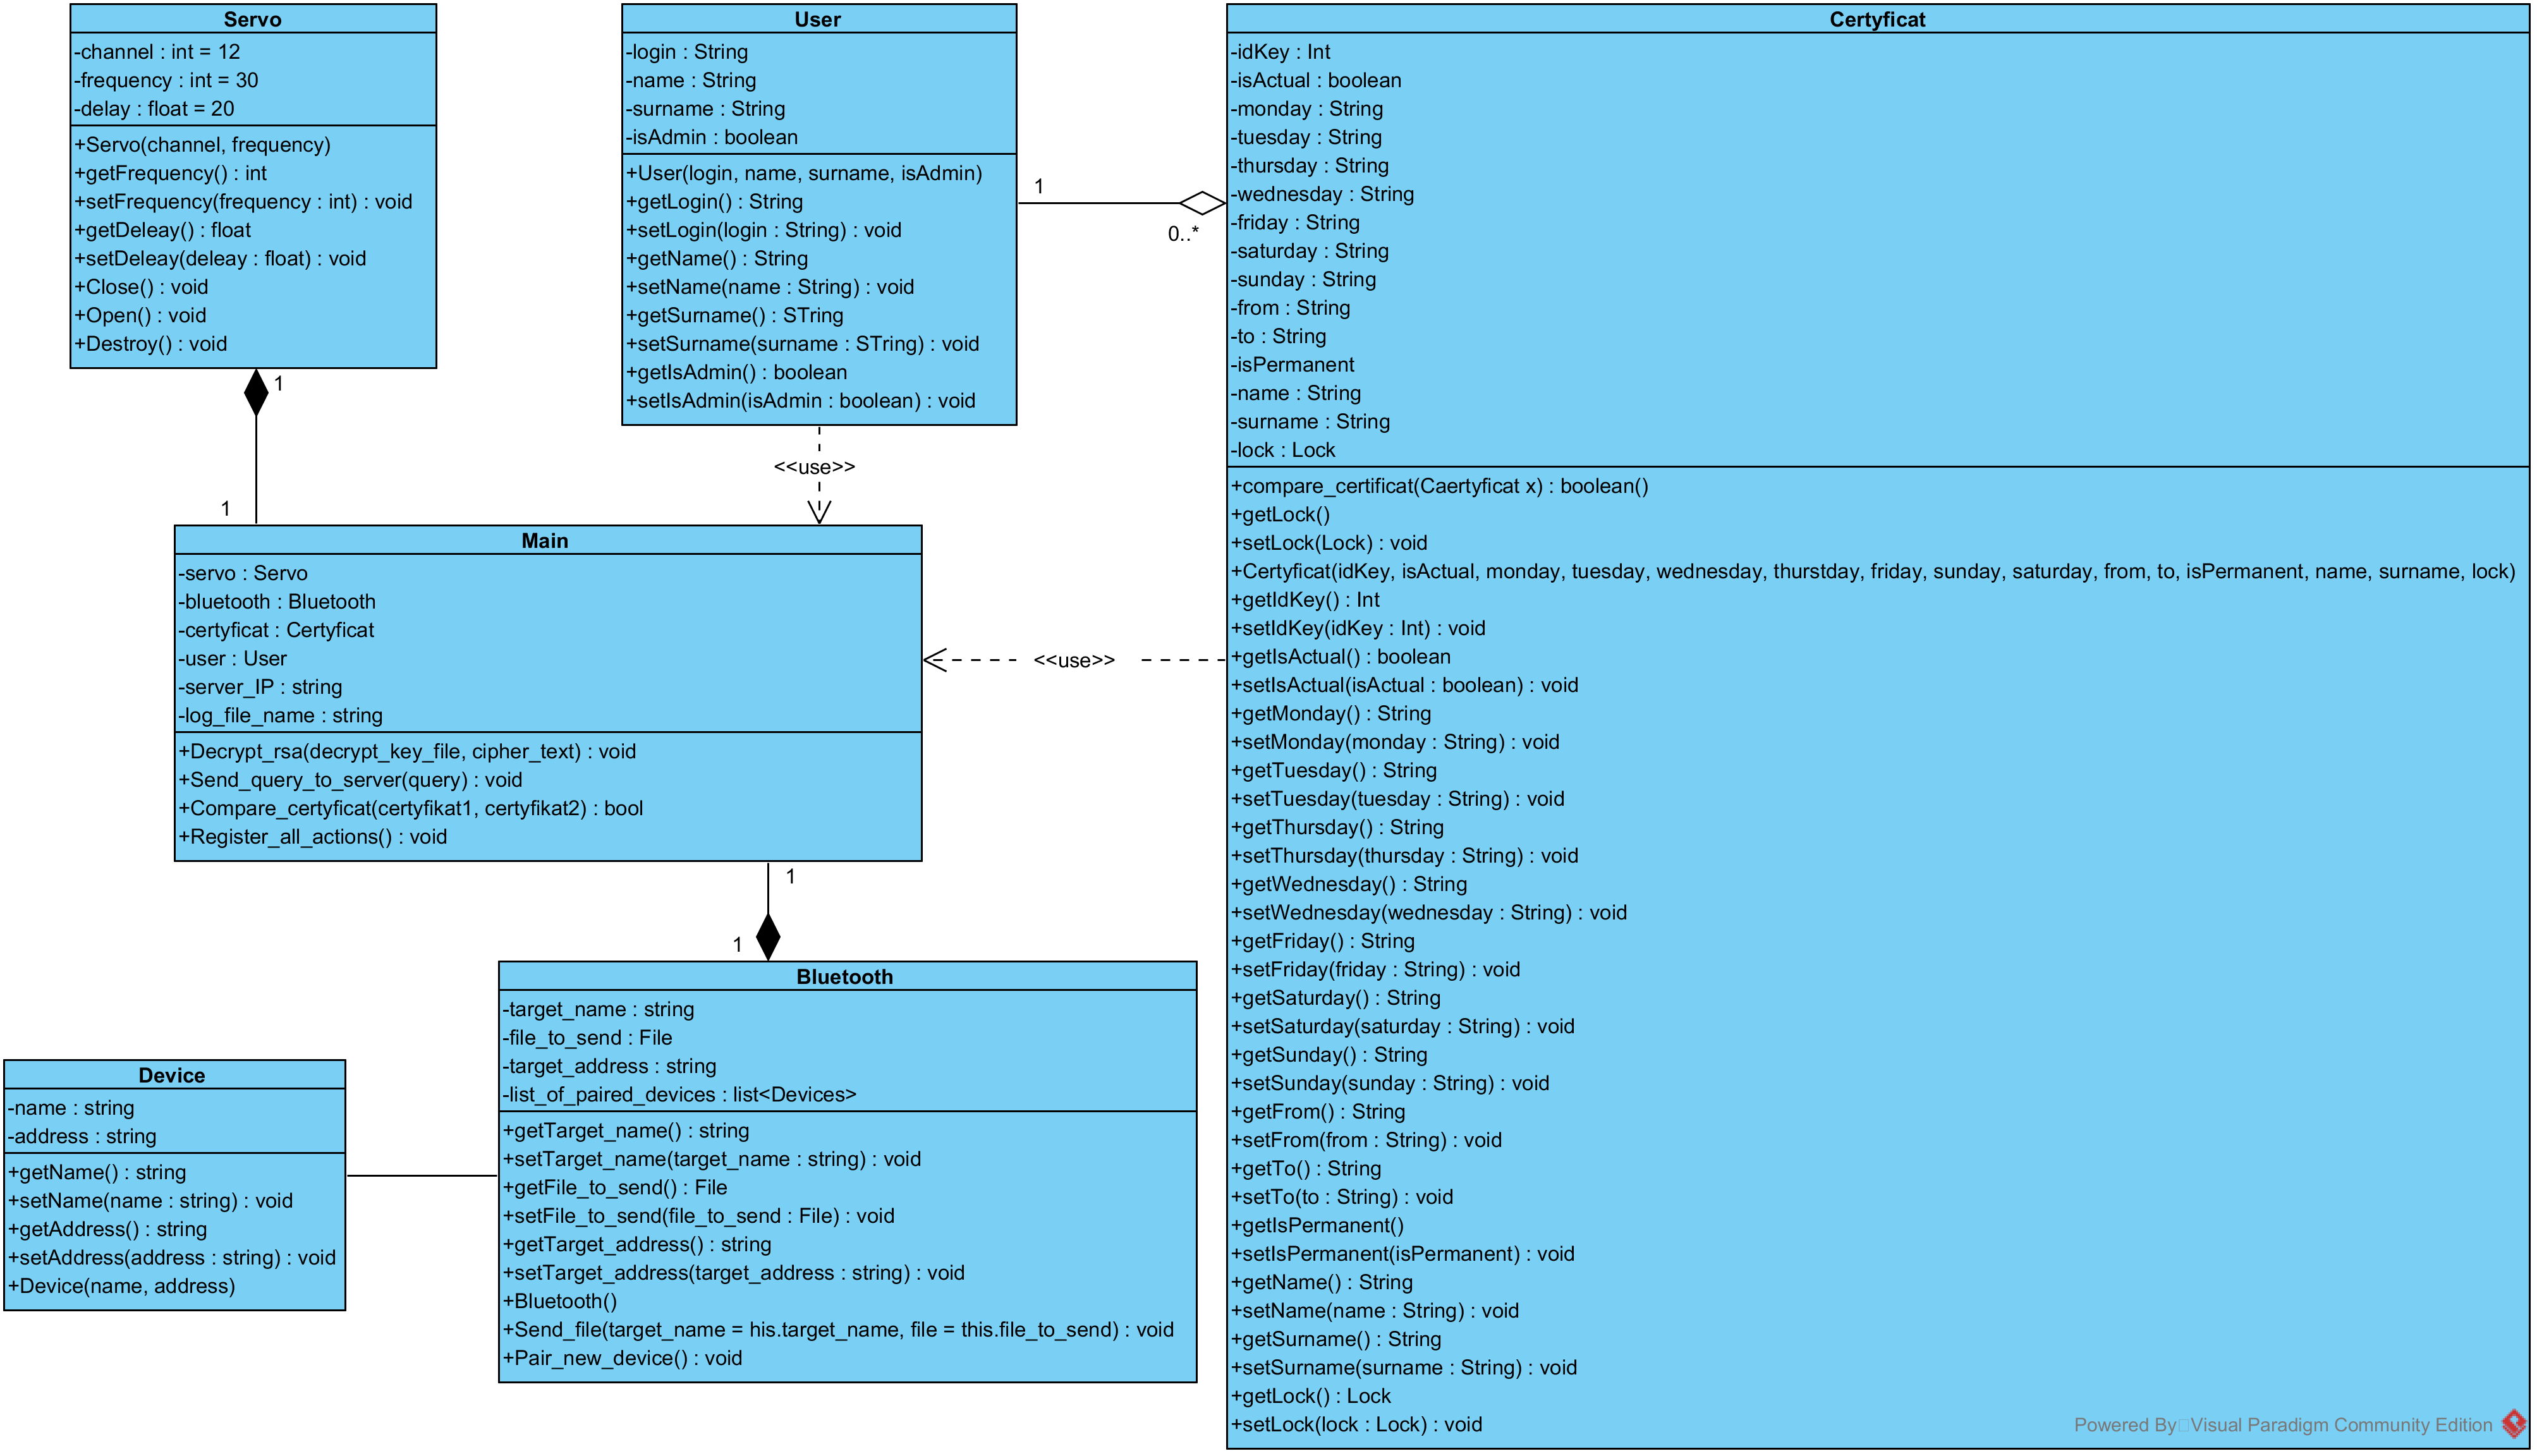
\includegraphics[width=16cm]{Obrazy/Diagram_klas_urzadzenie_sterujace.png}
		\caption{Diagram klas urządzenia sterującego}
		\label{diagram:Diagram_klas_urzadzenia_sterujacego}
	\end{figure}

		\begin{landscape}
		\begin{figure}[!h]
			\centering
			\vspace{2.5cm}
			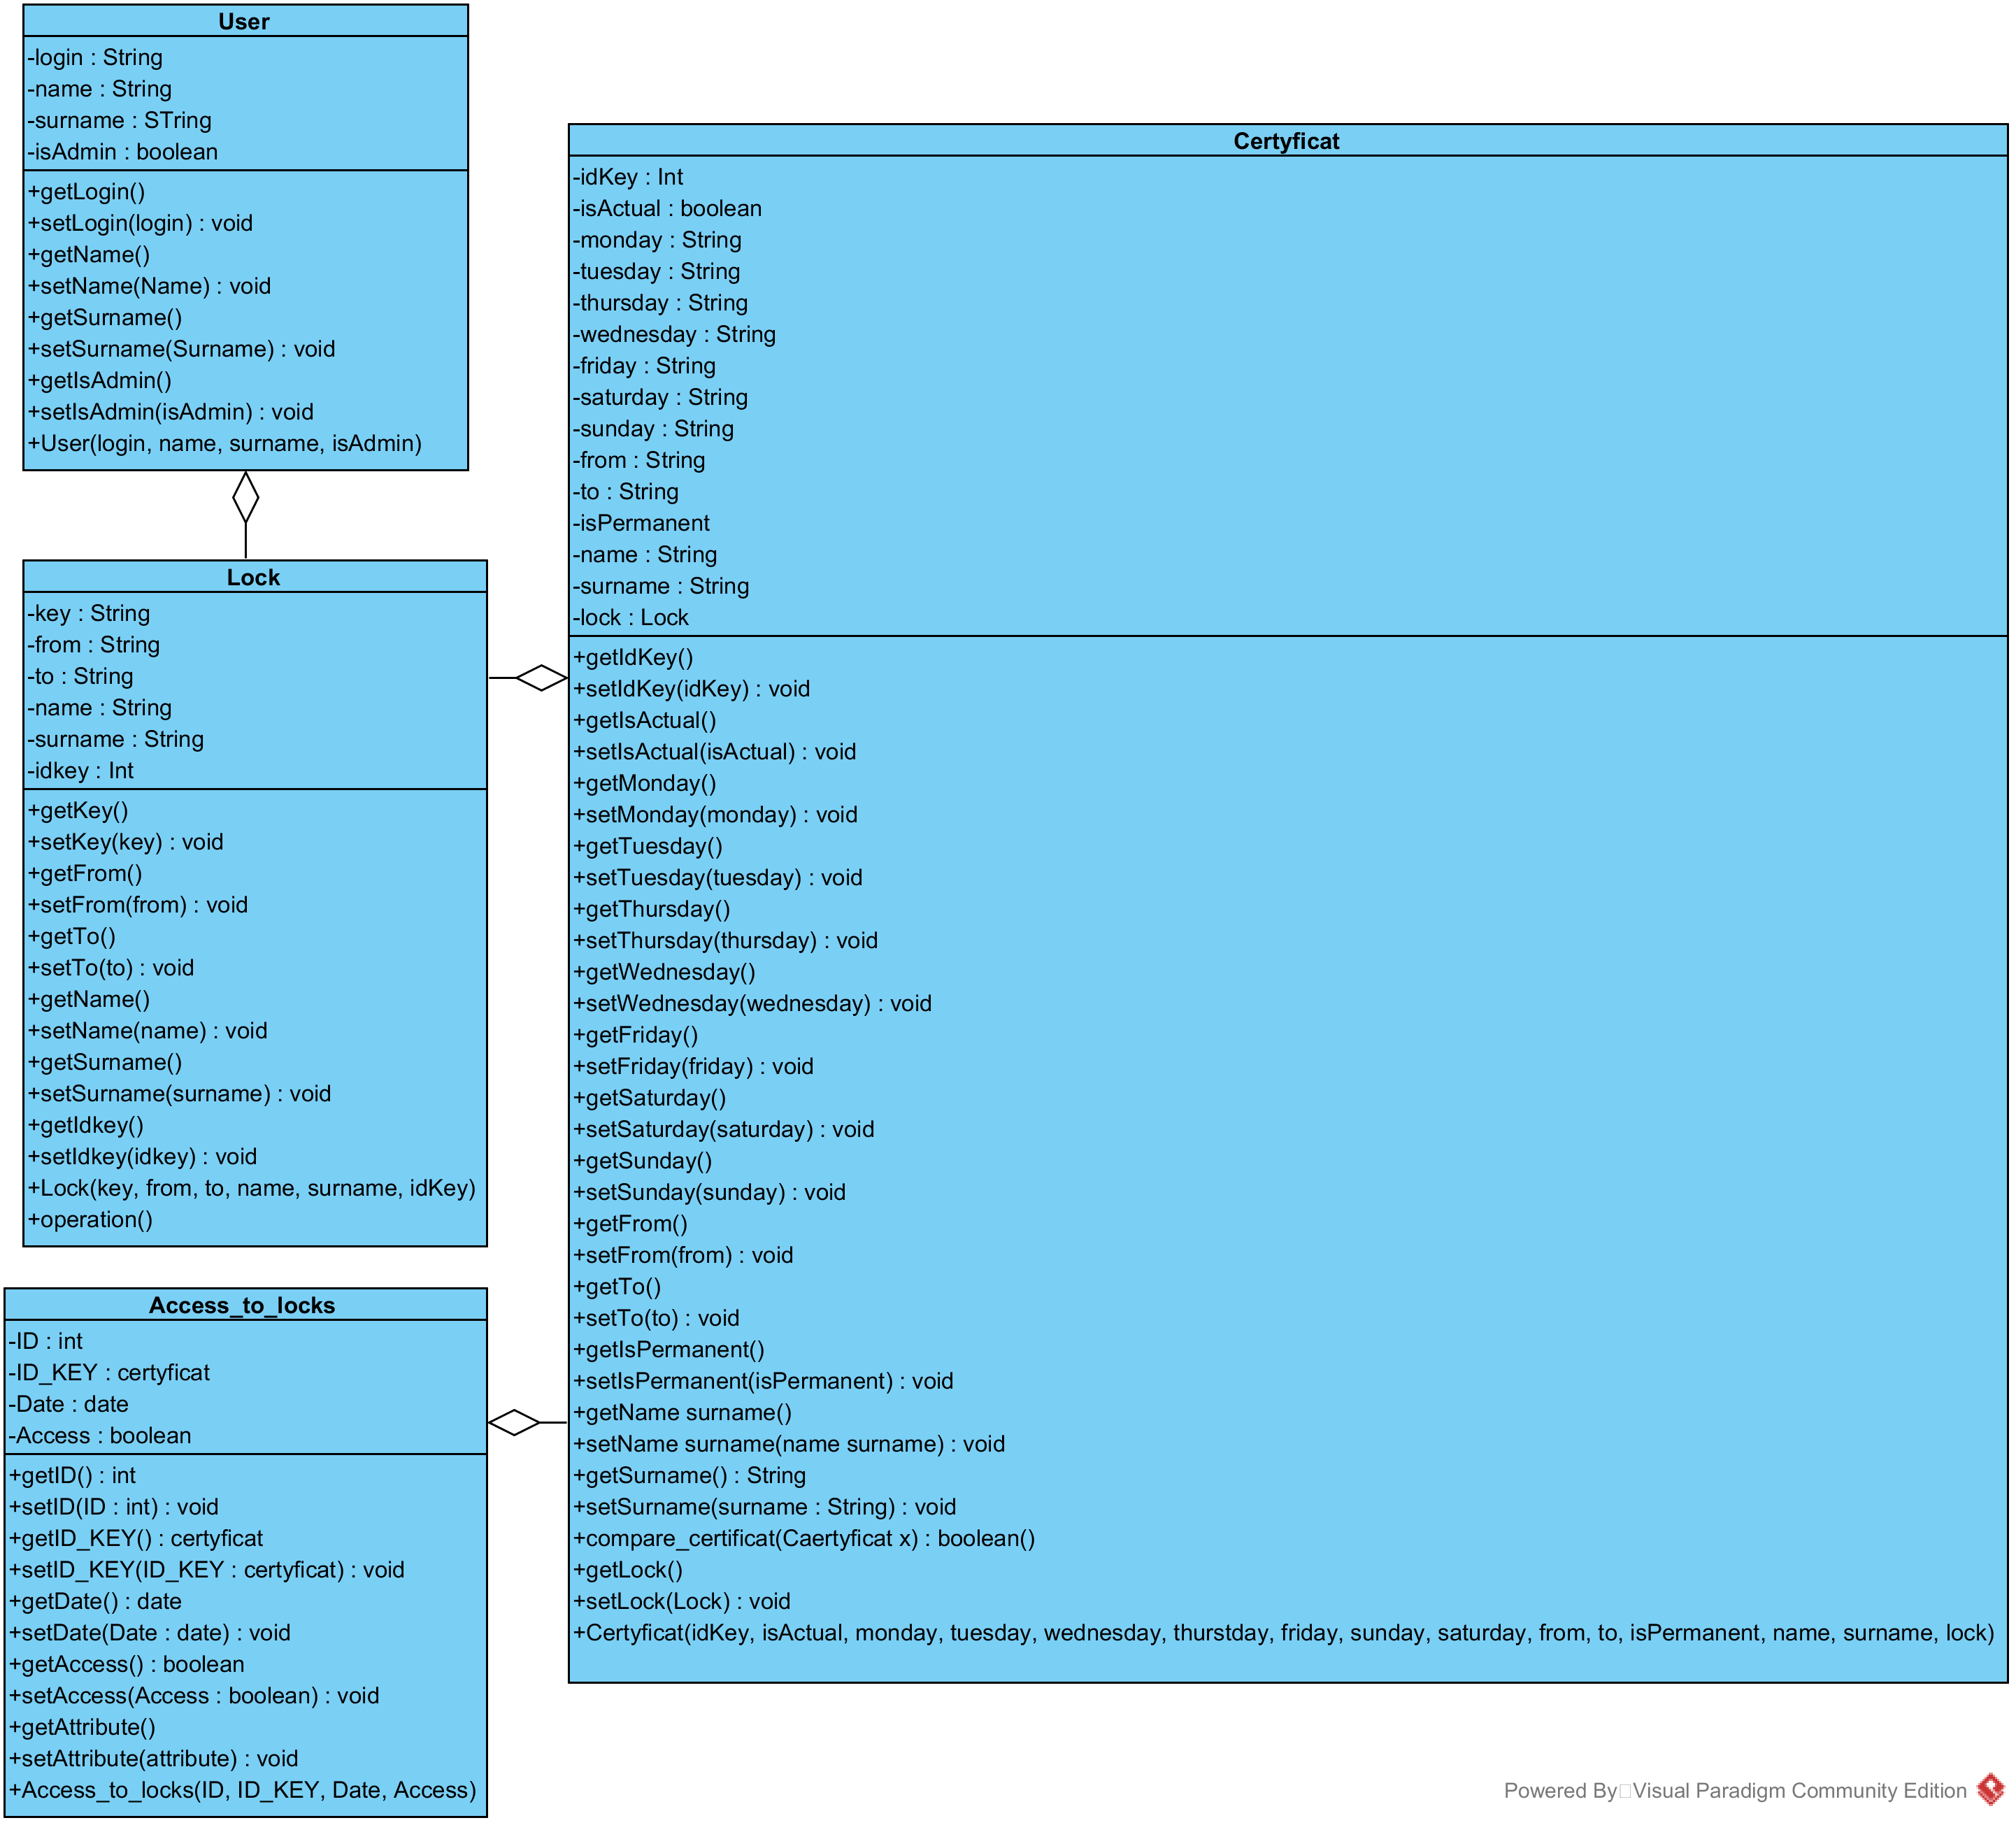
\includegraphics[width=24cm]{Obrazy/Diagram_klas_aplikacja_serwerowa.png}
			\caption{Diagram klas aplikacji serwerowej}
			\label{diagram:Diagram_klas_aplikacji_serwerowej}
		\end{figure}	
	\end{landscape}
			
	\paragraph{Moduł zliczania osób [Maciej Marciniak]}
	Moduł zliczania osób ze względu na swoją funkcjonalność i wykorzystanie biblioteki Open-CV nie wymaga tworzenia specjalnych klas, ani wyszczególnienia konkretnych metod. Jedyną możliwością jest wyodrębnienie klas przechowujących zliczane osoby znajdujące się w obiektywie kamery. Klasa dla konkretnej osoby posiadać ma metody do aktualizacji współrzędnych danej osoby oraz określające, czy przesuwa się w górę, czy w dół granicy obiektywu. Zmienne ''x'' i ''y'' przechowywać mają współrzędne osoby, ''donę'' oznaczać ukończenie śledzenia osoby, ''state'' obecny stan, a ''age'' i ''max\_age'' określać mają jak długo dany obiekt ma być namierzany.
	\begin{figure}[!h]
		\centering
		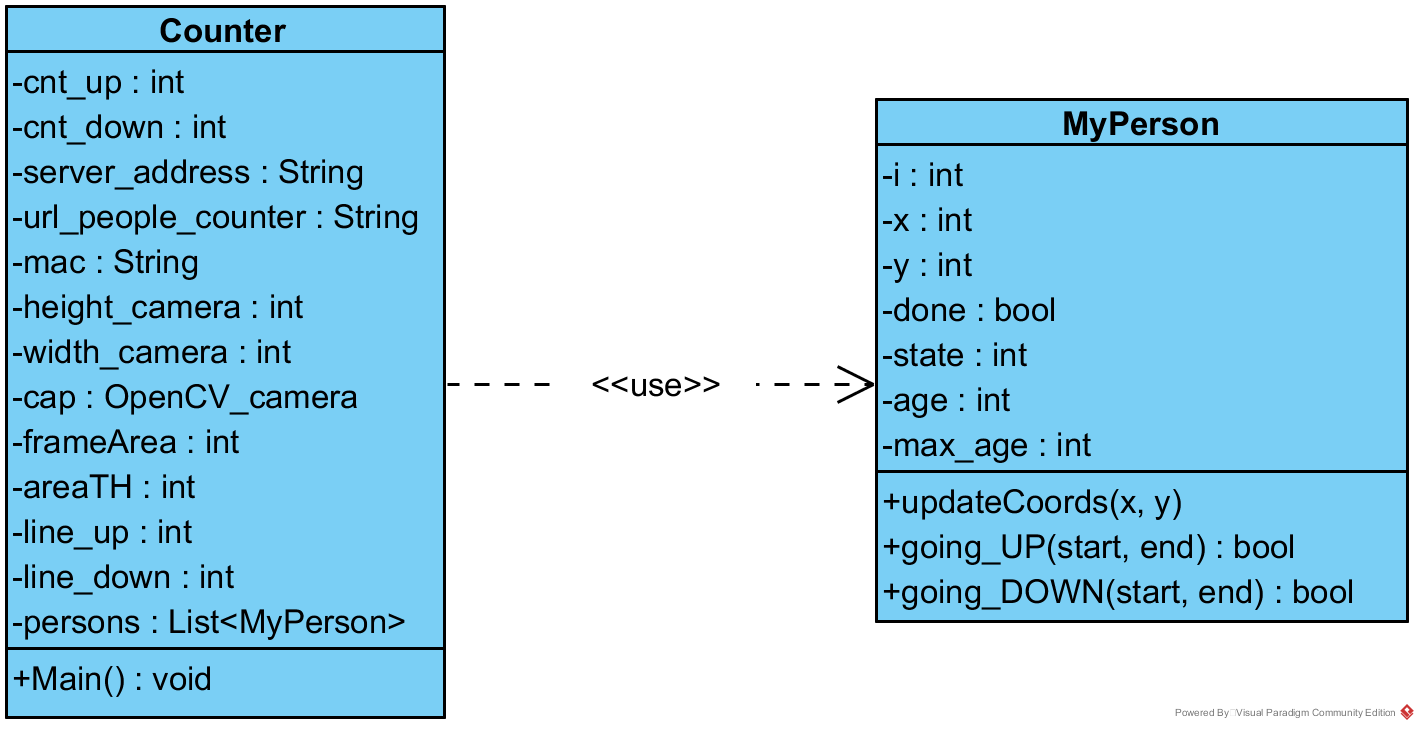
\includegraphics[width=12.5cm]{Obrazy/Diagram_klas_modul_zliczania_osob.png}
		\caption{Diagram klas modułu zliczania osób}
		\label{diagram:Diagram_klas_modul_zliczania_osob}
	\end{figure}
		
\subsection{Schemat elektryczny systemu [Maciej Marciniak]}\label{sec:Schemat elektryczny zamka}
Urządzenie sterujące jest jedynym fizycznym elementem projektowanym w~pracy dyplomowej. Uproszczony schemat instalacji elektrycznej przedstawiony został na Rys. \ref{schemat:schemat elektryczny systemu}. Centrum modułu jest mikrokomputer Raspberry Pi 3, zasilane z uniwersalnego gniazda USB. Zatem układ zasilany może być z komputera lub z zasilacza o napięciu 5V i minimalnym prądzie 1A. Urządzenie zostało zaprojektowane w taki sposób, aby można było podłączyć serwomechanizm i/lub elektrozamek. Umożliwia to dowolną konfigurację sprzętu według potrzeb i możliwości danych drzwi. 

Zasilanie elektrozamka realizowane jest z zasilacza 12V będącego w stanie podać dużą wartość prądu. Wysokie wymagania związane są z trudem wprawienia zapadki elektrozamka w ruch, ponieważ w tego typu urządzeniach często znajdują się elektromagnesy niewielkich rozmiarów. Ze względu na wyższe napięcie zasilania zamka niż dostarczane przez Raspberry Pi wymagane jest użycie tranzystora kluczującego prąd z zasilacza. Zdecydowano użyć elementu o oznaczeniu BD137-16 ze względu na swój niewielki koszt oraz wysoki prąd przewodzenia. Układ związany z serwomechanizmem jest zgodny z parametrami mikrokomputera, dlatego zasilanie oraz sterowanie prowadzone jest bezpośrednio z niego.

Piny sterujące urządzeniami w zamku są uzależnione od pełnionych w Raspberry Pi funkcji. Sterowanie elektrozamkiem możliwe jest przy użyciu niemal każdego pinu, ze względu na brak wymagań specjalistycznego sterowania, za to serwomechanizm wymaga zastosowania sygnału PWM, który musi być obsługiwany przez konkretny GPIO (w tym wypadku takim pinem jest GPIO\_18).\cite{RP3}
\newpage
\begin{figure}[!h]
	\centering
	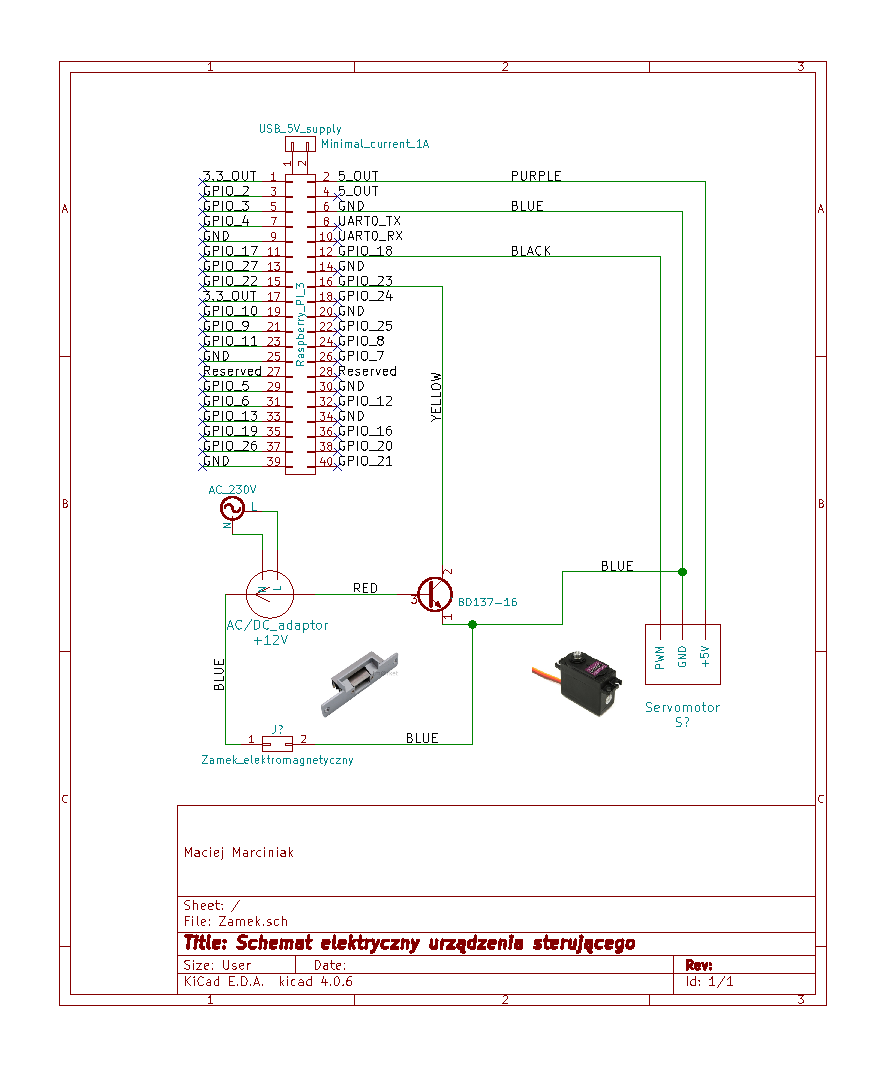
\includegraphics[width=17cm]{Obrazy/Schemat_elektryczny.pdf}
	\caption{Schemat elektryczny systemu}
	\label{schemat:schemat elektryczny systemu}
\end{figure}
\newpage

\subsection{Komunikacja modułów systemu z aplikacją  serwera [Maciej Marciniak]}\label{Komunikacja serwer}
Tworząc aplikację serwerową należy zapewnić możliwość komunikację (tak zwane API), która pozwoli na interakcję z zasobami zarządzanymi przez serwer. Przedstawiany system udostępniać powinien usługi dla urządzenia sterującego, w tym również modułu zliczającego osoby oraz dla aplikacji mobilnej. Ze względu na odległości mogące dzielić systemy od siebie zdecydowano ,jako interfejs komunikacji sieć Internetową z użyciem bezpiecznego protokołu Https. 
	\subsubsection{Komunikaty HTTPRequest pomiędzy urządzeniem sterującym, a serwerem}
	Komunikacja pomiędzy urządzeniem sterującym, a serwerem powinna  zapewniać możliwość weryfikacji poprawności certyfikatów dostępowych oraz szyfrujących w celu potwierdzenia tożsamości użytkownika oraz zdecydowaniu, czy dana osoba ma przydzielony dostęp do pomieszczenia o danej porze dnia. Dodatkowo serwer powinien udostępniać API do wpisywania liczby osób w~pomieszczeniu oraz wpisujące do bazy danych, czy dostęp został przyznany, czy nie. Wykaz wymaganych API znajduje się w Tabeli \ref{tab:http_raspberry}.
	\subsubsection{Komunikaty HTTPRequest pomiędzy aplikacją mobilną, a serwerem}
	Aplikacja mobilna powinna posiadać podstawowe operacja użytkowników, takie jak logowanie, rejestracja, wylogowanie, dodatkowo powinny zostać udostępnione funkcje związane z zarządzaniem konta jak i certyfikatami dostępowymi. Funkcjonalności powiązane z operacjami na koncie to zmiana hasła, wymiana certyfikatu szyfrującego, możliwość blokowania konta. Funkcja zarządzającymi certyfikatami dostępowymi są generowanie nowych kluczy, blokowanie ich, aktywowanie. API powinno być dedykowane dla dwóch rodzajów użytkowników zwykłego oraz z uprawnieniami administratora. Właściwości funkcji drugiego typu konta powinny dodatkowo udostępniać podgląd w historię używania poszczególnych zamków oraz edycję wszystkich parametrów kont użytkownika zwykłego. Wykaz zaprojektowanego API znajduje się w Tabeli \ref{tab:http_mobilne}.\cite{programowanie_aplikacji_webowych}
	\begin{landscape}
		\begin{longtable}[!ht]{|m{5cm}|m{7cm}|m{4.5cm}|m{5.5cm}|} 
			\caption{Tabela komunikatów HTTP dla Raspberry Pi}
			\label{tab:http_raspberry}\\
			\hline	
			Adres URL & Parametry & Odpowiedź & Opis \\	\hline
			/api/RPI/download/certificate/ & certificate\_id --- identyfikator certyfikatu, \newline RPI\_MAC --- adres MAC urządzenia, \newline login\_user --- login użytkownika & ''data'': dict\_all\_certificate, \newline ''public\_key'': public\_key \tablinia ''data'': ''invalid'' & Pobranie certyfikatu użytkownika \\ \hline
			/api/RPI/access\_decision/ & certificate\_id --- identyfikator certyfikat,u \newline decision --- informacja o odmowie/akceptacji dostępu & ''status'': ''ok'' \tablinia ''data'': ''invalid'' & Informacja do serwera o statusie otwierania zamka \\ \hline
			/api/RPI/people\_counter/ & counter --- liczba osób w pomieszczeniu, \newline RPI\_MAC --- adres MAC urządzenia & ''status'': ''ok'' \tablinia ''data'': ''Invalid'' & Ustawienie licznika osób w pomieszczeniu \\ \hline
		\end{longtable}
	\end{landscape}

\begin{landscape}
	\begin{longtable}[!ht]{|m{5cm}|m{6.5cm}|m{5cm}|m{5.5cm}|} 
		\caption{Tabela komunikatów HTTP dla urządzenia mobilnego}
		\label{tab:http_mobilne}\\
		\hline	
		Adres URL & Parametry & Odpowiedź & Opis \\	\hline
		/api/login/ & username --- login użytkownika, \newline password --- hasło użytkownika & ''status'': ''ok'', ''token'': token \tablinia ''status'':''ERROR~\mbox{PASSWORD}'', ''token'': ''invalid'' \tablinia ''status'': ''not activated'', \newline ''token'': ''invalid'', \tablinia ''status'': ''blocked'', \newline''token'': ''invalid'' & Logowanie użytkownika do aplikacji \\ \hline
		/api/register/ & login --- login użytkownika, \newline password --- hasła użytkownika, \newline name --- imię użytkownika, \newline surname -- nazwisko użytkownika, \newline publickey --- klucz publiczny użytkownika & ''status'': 'ERROR'' \tablinia ''status'': ''REGISTER OK'' & Rejestracja nowego użytkownika do aplikacji \\ \hline
		/api/logout/ & login --- login użytkownika, \newline token --- klucz sesji logowania & ''status'': ''logout'' \tablinia ''status'': ''invalid'' & Wylogowanie użytkownika z aplikacji \\ \hline
		/api/download/all\_certifacate/ & login --- login użytkownika, \newline token --- klucz sesji logowania & ''data'': dict\_all\_certificate \tablinia ''status'': ''invalid'' & Pobranie wszystkich dostępnych certyfikatów użytkownika \\ \hline
		/api/download/all\_locks/ & login --- login użytkownika, \newline token --- klucz sesji logowania & ''data'': dict\_all\_locks \tablinia ''status'': ''invalid'' & Pobranie listy wszystkich dostępnych zamków w systemie \\ \hline
		/api/download/all\_user/ & login --- login użytkownika, \newline token --- klucz sesji logowania & ''data'': dict\_all\_users \tablinia ''status'': ''invalid'' & Pobranie listy wszystkich użytkowników systemu \\ \hline
		/api/deactivation/ & login --- login użytkownika, \newline token --- klucz sesji logowania, \newline certificate\_id --- identyfikator certyfikatu do usunięcia & ''status'': ''ok'' \tablinia ''status'': ''invalid'' & Usunięcie dostępu do certyfikatu \\ \hline
		/api/request\_new\_certificate/ & login --- login użytkownika, \newline token --- klucz sesji logowania, \newline lock\_id --- identyfikator zamka & ''status'': ''ok'' \tablinia ''status'': ''invalid'' & Wnioskowanie o nowy certyfikat \\ \hline
		/api/change\_password/ & login --- login użytkownika, \newline token --- klucz sesji logowania, \newline newpasswd --- nowe hasło użytkownika & ''status'': ''ok'' \tablinia ''status'': ''invalid'' & Zmiana hasła użytkownika \\ \hline
		/api/replace\_certificate/ & login --- login użytkownika, \newline token --- klucz sesji logowania, \newline old\_public\_key --- obecny klucz publiczny użytkownika, \newline new\_public\_key --- nowy klucz publiczny użytkownika & ''status'': ''ok'', \newline ''data'': dict\_certificate \tablinia ''status'': ''invalid'' & Wymiana certyfikatu szyfrującego na żądanie użytkownika \\ \hline
		/api/admin/history/ & login --- login użytkownika, \newline token --- klucz sesji logowania & ''data'': dict\_history \tablinia ''status'': ''invalid'' & Pobranie historii użycia zamków w systemie (administrator) \\ \hline
		/api/admin/download/\linebreak all\_certificate/ & login --- login użytkownika, \newline token --- klucz sesji logowania & ''data'': dict\_all\_certificate \tablinia ''status'': ''invalid'' & Pobranie wszystkich certyfikatów z systemu (administrator)\\ \hline
		/api/admin/deactivation/ & login --- login użytkownika, \newline token --- klucz sesji logowania, \newline certificate\_id --- identyfikator certyfikatu do usunięcia & ''status'': ''ok'' \tablinia ''status'': ''invalid'' & Usunięcie dostępu do certyfikatu (administrator) \\ \hline
		/api/admin/register\_waiting/ & login --- login użytkownika, \newline token --- klucz sesji logowania & ''status'': ''ok'' \tablinia ''status'': ''invalid'' & Pobranie listy oczekujących użytkowników na zaakceptowanie rejestracji \\ \hline
		/api/admin/register\_decision/ & login --- login użytkownika, \newline token --- klucz sesji logowania, \newline user\_login --- login użytkownika, którego dotyczy decyzja, \newline decision --- decyzja True/False dotycząca akceptacji rejestracji & ''status'': ''ok'' \tablinia ''status'': ''invalid'' & Podjęcie decyzji przez administratora dotycząca rejestracji użytkownika o danym loginie \\ \hline
		/api/admin/certificate\_waiting/ & login --- login użytkownika, \newline token --- klucz sesji logowania & ''status'': ''ok'' \tablinia ''status'': ''invalid'' & Pobranie listy oczekujących certyfikatów na zaakceptowanie \\ \hline
		/api/admin/certificate\_decision/ & login --- login użytkownika, \newline token --- klucz sesji logowania, \newline certificate\_id --- identyfikator certyfikatu, którego dotyczy decyzja & ''status'': ''ok'' \tablinia ''status'': ''invalid'' & Podjęcie decyzji przez administratora dotycząca przyjęcia \\ \hline
		/api/admin/\-generate\_new\_certificate/ & login --- login użytkownika, \newline token --- klucz sesji logowania, \newline user\_id --- identyfikator użytkownika, \newline lock\_id --- identyfikator zamka, \newline from\_date --- data od której obowiązuje certyfikat, \newline to\_date --- data do której obowiązuje certyfikat, \newline monday...sunday --- 7 parametrów oznaczjacych zakresy godzin w poszczególnych dniach tygodnia, \newline is\_pernament --- czy dostęp jest ciągły, \newline name --- imię użytkownika certyfikatu, \newline surname --- nazwisko użytkownika certyfikatu & ''status'': ''ok'' \tablinia ''status'': ''invalid'' & Generowanie nowego certyfikatu (administrator) \\ \hline
		/api/admin/\-deactivation\_user\_accout/ & login --- login użytkownika, \newline token --- klucz sesji logowania, \newline user\_id --- identyfikator użytkownika, którego konto ma zostać zablokowane & ''status'': ''ok'' \tablinia ''status'': ''invalid'' & Zablokowanie konta wybranego użytkownika (administrator) \\ \hline
		/api/admin/deactivation\-\_user\_certificate/ & login --- login użytkownika, \newline token --- klucz sesji logowania, \newline user\_id --- identyfikator użytkownika, którego certyfikat szyfrujący ma zostać zablokowany & ''status'': ''ok'' \tablinia ''status'': ''invalid'' & Zablokowanie certyfikatu szyfrującego wybranego użytkownika (administrator) \\ \hline
	\end{longtable}\cite{programowanie_aplikacji_webowych}
\end{landscape}
\newpage
\subsection{Interfejs komunikacji pomiędzy urządzeniem sterującym i aplikacją mobilną [Maciej Marciniak]}
W rozdziale \ref{Komunikacja serwer} opisano dwie ścieżki komunikacji urządzeń z serwerem, trzecią opcją jest komunikacja pomiędzy urządzeniem sterującym, a aplikacją mobilną. W tym wypadku nie jest istotna duża odległość komunikacji, wręcz jest niewskazana. Odpowiednim interfejsem, zapewniającym szybką i uniwersalną transmisję jest moduł bluetooth, w który wersja mikrokomputera Raspberry Pi 3 jest wyposażona. 

Komunikacja pomiędzy urządzeniami polega tylko na przesyle podpisanych cyfrowo certyfikatów dostępowych. Format przesyłanych danych jest w postaci: \\
\begin{minipage}[t]{8cm}
	<id~certyfikatu>;\\<login~użytkownika>;\\<sygnatura~klucza~dostępowego>;\\<certyfikat~szyfrujący~w~postaci~JSONa>
\end{minipage} 

\subsection{Interfejs graficzny systemu [Damian Filipowicz]}\label{sec:Projekt interfejsu graficznego}
Jednym z dwóch modułów posiadających w systemie interfejs graficzny jest aplikacja mobilna, drugim zaś strona internetowa. Aplikacja mobilna zawierać powinna wszystkie funkcjonalności systemu z wykorzystaniem czytelnego interfejsu użytkownika. Strona internetowa  ma mieć na celu interakcję tylko z administratorem systemu, dlatego nie są stawiany wysoki priorytet estetyczny. Nominalną wielkością ekranu braną pod uwagę przy projektowaniu interfejsu graficznego dla aplikacji mobilnej będzie ekran o wielkości 5 in. Motywacją takiego wyboru jest rozkład popularności ekranów dla urządzeń mobilnych w 2017 roku. Jak widać na załączonym rysunku (rys. \ref{rys:prognoza}) wielkość ekranu 5,0 jest pierwszą znaczącą wielkością dla urządzeń mobilnych\footnote{ \href{https://www.idc.com/getdoc.jsp?containerId=prUS42628117}{https://www.idc.com/getdoc.jsp?containerId=prUS42628117} (odczyt z dnia 24.01.2018)}. 
	\begin{figure}[ht!]
	\centering
	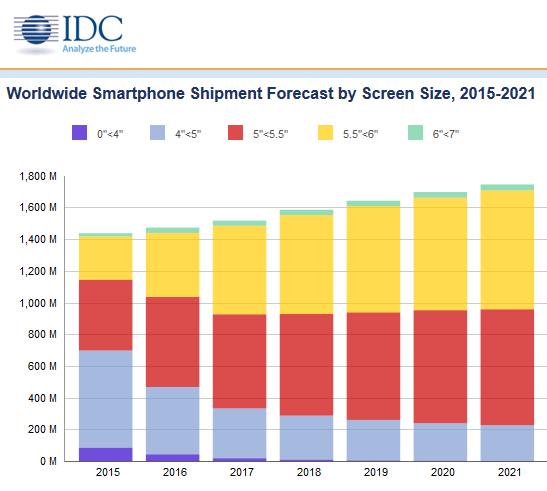
\includegraphics[width=13cm]{Obrazy/porowananie}
	\caption{Prognoza popularności wielkości ekranów dla urządzeń mobilnych na przestrzeni lat 2015-2021}
	\label{rys:prognoza}
\end{figure}

	\subsubsection{Widoki aplikacji mobilnej}
	\paragraph*{Panel logowania użytkownika}
	Widok umożliwiać będzie zalogowanie się użytkownika do systemu poprzez podanie loginu, hasła oraz adres IP serwera w odpowiednie pola, a następnie kliknięcie w przycisk ''ZALOGUJ SIĘ”. Samo pole hasła będzie maskowane. Jeśli nie posiada się konta, zostanie utworzona możliwość  utworzenia konta poprzez przycisk ''ZAREJESTRUJ SIĘ”. (Rys. \ref{rys:panel_logowania_pionowo})
	
	\begin{figure}[ht!]
		\begin{minipage}{0.45\textwidth}
			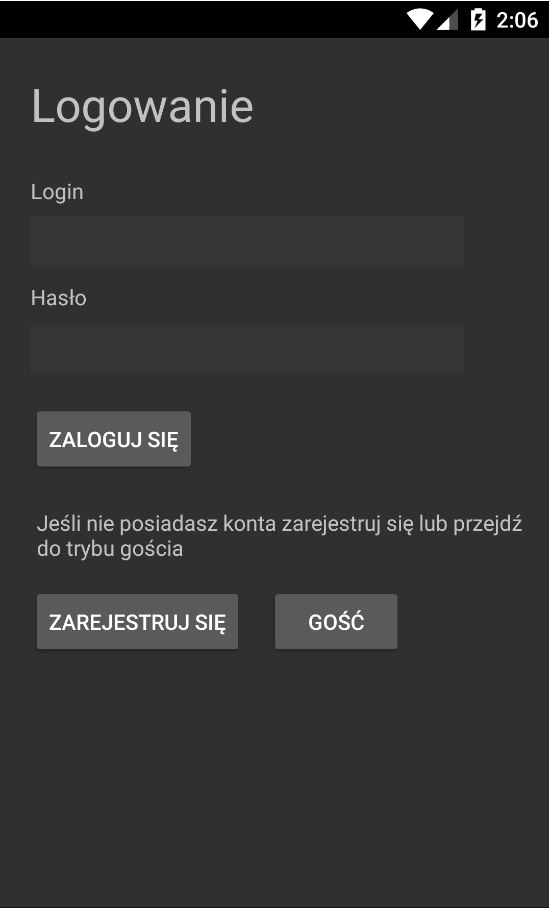
\includegraphics[width=\textwidth]
			{Obrazy/logowanie_uzytkownika_pionowo}
			\caption{Panel logowania użytkownika}
			\label{rys:panel_logowania_pionowo}
		\end{minipage}
		\hspace{0.1\textwidth}
		\begin{minipage}{0.45\textwidth}
			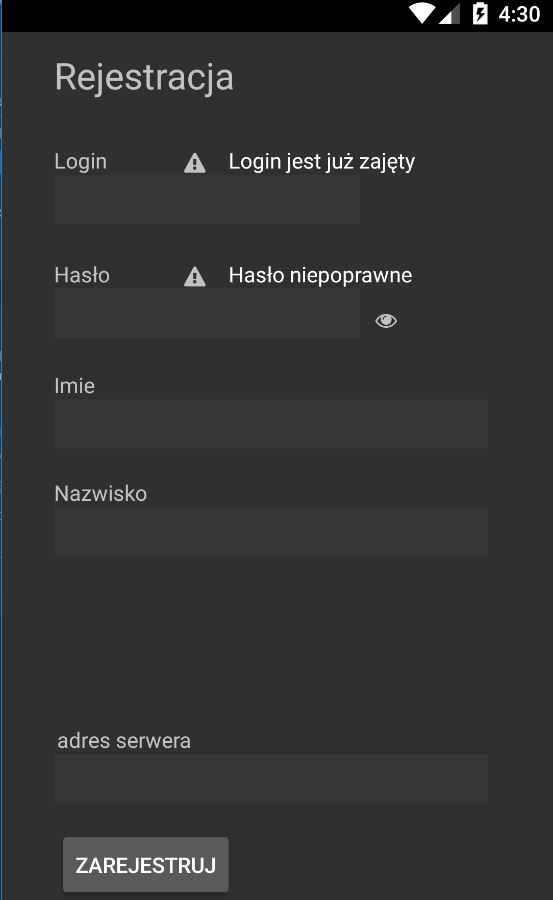
\includegraphics[width=\textwidth]{Obrazy/rejestracja_uzytkownika_pionowo}
			\caption{Panel logowania użytkownika }
			\label{rys:panel_rejestracji_pionowo}
		\end{minipage}	
	\end{figure}

	\paragraph*{Panel rejestracji użytkownika}
	Panel rejestracji służyć będzie do utworzenie nowego użytkownika poprzez podanie loginu, hasła, imienia i nazwiska użytkownika oraz adresu IP serwera do którego chcemy się zarejestrować. Pole z hasłem będzie maskowane wraz z możliwością odkrywania hasła przy pomocy ikonki oko Po upewnieniu się, że wszystkie dane są poprawne, aby zakończyć proces rejestracji, trzeba będzie kliknąć przycisk ''ZAREJESTRUJ”. (Rys. \ref{rys:panel_rejestracji_pionowo})

	\newpage
	\paragraph*{Panel listy zamków}
	Widok listy dostępnych zamków przedstawia listę nazw zamków do jakich dany użytkownik ma dostęp. Ułatwieniem będzie możliwość sortowania wyników i wyszukiwanie po nazwach. Kliknięcie w nazwę zamka spowoduje otwarcie zamka. Zmiana koloru\footnote{ Opisy znaczeń poszczególnych kolorów oraz symboli opisane są w rozdziale \ref{Symbolika ikon}} ikon zamków sygnalizować będzie status zamka. (Rys. \ref{rys:panel_listy_dostepnych_zamkow_pionowo})
	
	\begin{figure}[ht!]
		\begin{minipage}{0.45\textwidth}
			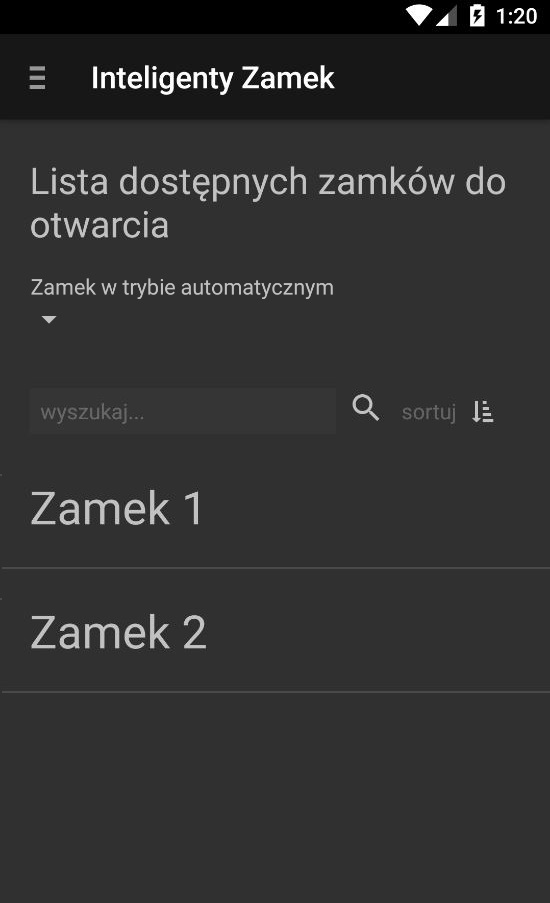
\includegraphics[width=\textwidth]
			{Obrazy/lista_dostepnych_zamkow_pionowo}
			\caption{Lista dostępnych zamków}
			\label{rys:panel_listy_dostepnych_zamkow_pionowo}
		\end{minipage}
		\hspace{0.1\textwidth}
		\begin{minipage}{0.45\textwidth}
			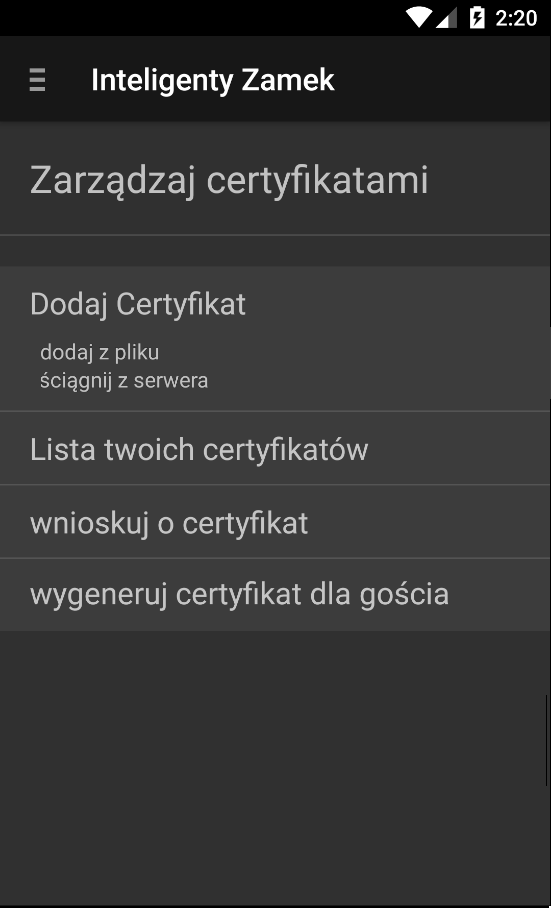
\includegraphics[width=\textwidth]{Obrazy/zarzadzaj_certyfikatami_pionowo}
			\caption{Panel zarządzania certyfikatami }
			\label{rys:panel_zarządzania_certyfikatami_pionowo}
		\end{minipage}	
	\end{figure}

	\paragraph*{Panel zarządzania certyfikatami}
Panel zarządzania certyfikatami umożliwi wybór funkcji dodania certyfikatu. Kolejne pozycje to lista posiadanych certyfikatów oraz wysłanie wniosku o utworzenie nowego certyfikatu  (Rys. \ref{rys:panel_zarządzania_certyfikatami_pionowo})
\newpage

	\paragraph*{Panel boczny}
	Panel boczny pozwalać będzie na szybkie przełączanie pomiędzy widokami. Chowany zostanie po lewej stronie ekranu. Umożliwi przechodzenie odpowiednio do listy zamków, zarządzania certyfikatami, panelu administracyjnego oraz ustawień. Ostatnia pozycja spowoduje wylogowanie z aplikacji. Pnanel ten w zależnośći od uprawnień użytkownika możę posiadać lub nie pole z panelem administraotra (Rys. \ref{rys:panel_boczny_pionowo} i \ref{rys:panel_boczny_pionowo2})
	
	\begin{figure}[ht!]
		\begin{minipage}{0.45\textwidth}
			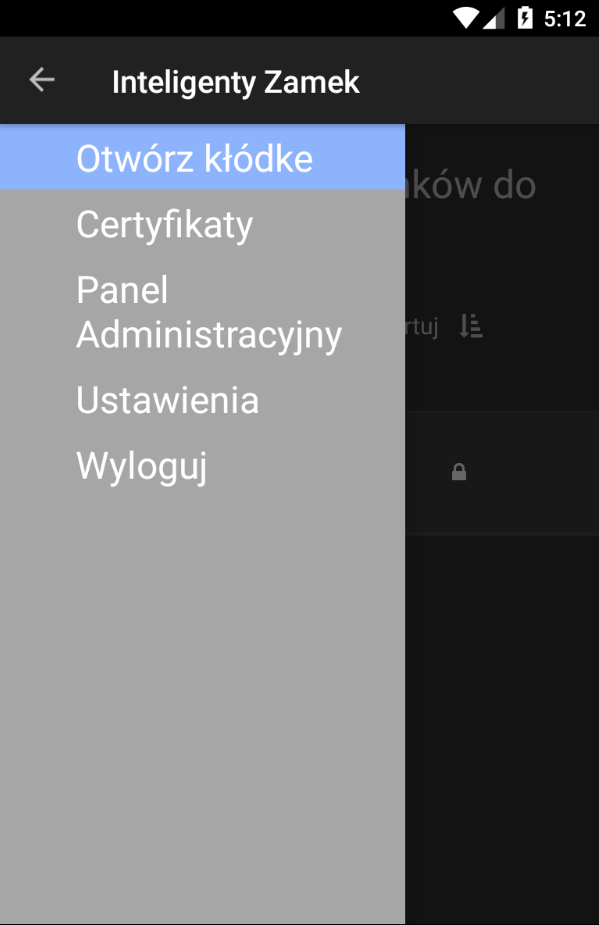
\includegraphics[width=\textwidth]
			{Obrazy/panel_boczny_pionowo}
			\caption{Panel boczny z uprawnieniami administratora}
			\label{rys:panel_boczny_pionowo}
		\end{minipage}
	\hspace{0.1\textwidth}
		\begin{minipage}{0.45\textwidth}
			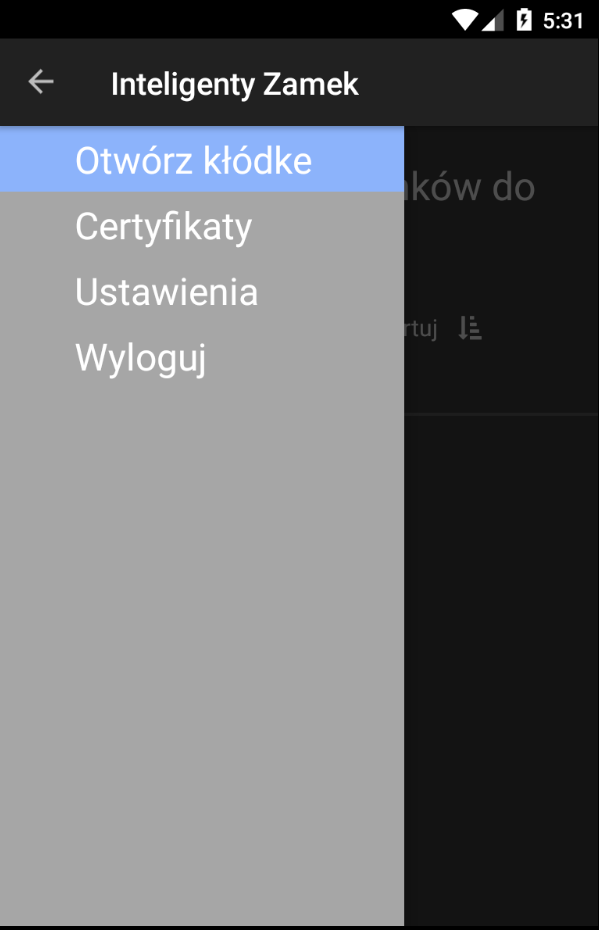
\includegraphics[width=\textwidth]{Obrazy/panel_boczny_pionowo2}
			\caption{Panel boczny bez uprawnieni administratora}
			\label{rys:panel_boczny_pionowo2}
		\end{minipage}	
	\end{figure}
\newpage
	
	\paragraph*{Panel listy certyfikatów}
	Panel listy certyfikatów, będzie listą aktualnych certyfikatów należących do użytkownika. Kliknięcie w dany certyfikat przeniesie do widoku szczegółowego związanego z operacjami na tym certyfikacie. (Rys. \ref{rys:panel_listy_certyfikatów_pionowo} )
	
	\begin{figure}[ht!]
		\begin{minipage}{0.45\textwidth}
			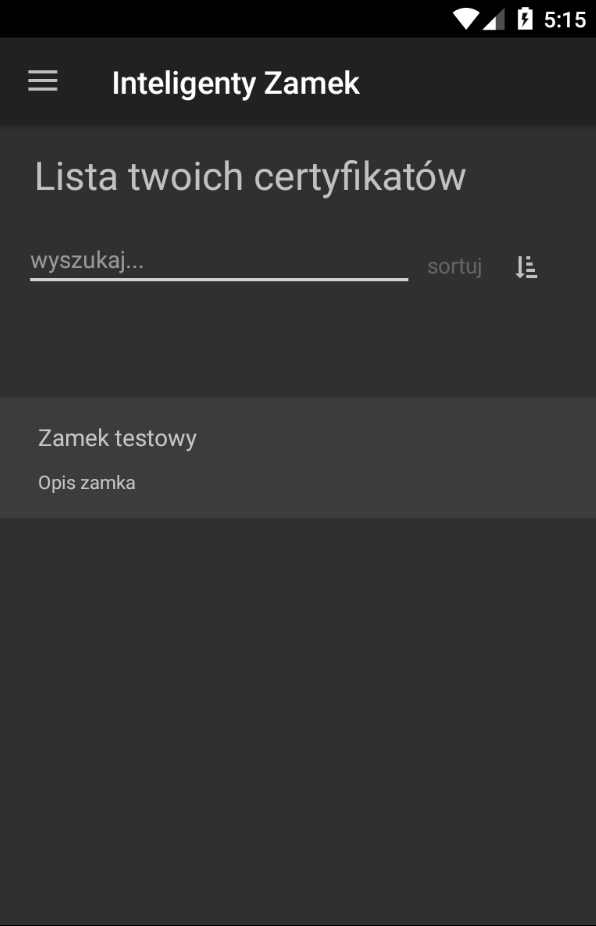
\includegraphics[width=\textwidth]
			{Obrazy/lista_certyfikatow_pionowo}
			\caption{Panel listy certyfikatów}
			\label{rys:panel_listy_certyfikatów_pionowo}
		\end{minipage}
		\hspace{0.1\textwidth}
		\begin{minipage}{0.45\textwidth}
			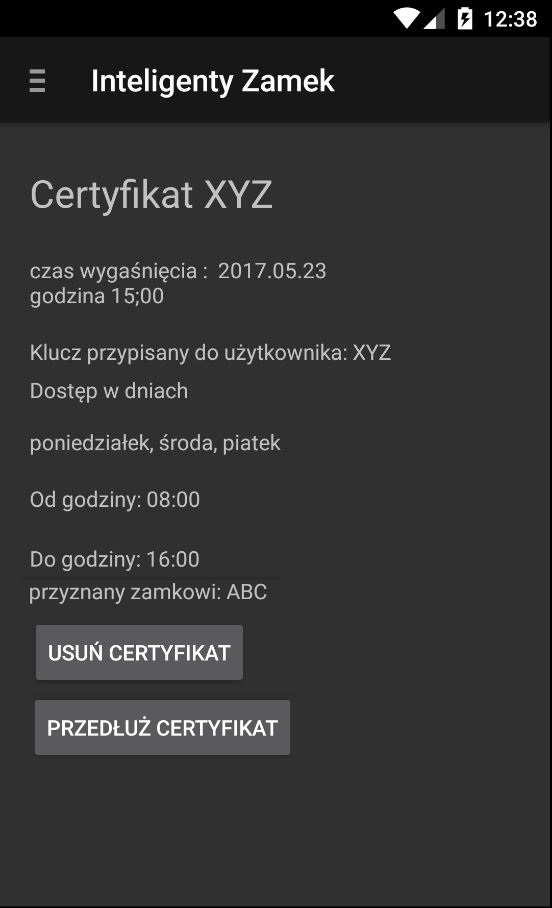
\includegraphics[width=\textwidth]{Obrazy/certyfikat_pionowo}
			\caption{Panel certyfikatu }
			\label{rys:panel_certyfikatu_pionowo}
		\end{minipage}	
	\end{figure}

	\paragraph*{Panel certyfikatu}
	Panel certyfikatu zawierać będzie informacje o dacie wygaśnięcia, którego zamku dotyczy oraz w jakim czasie przyznaje dostęp. Na dole dostępne będą dwa przyciski pozwalające usunąć certyfikat lub wysłać prośbę o przedłużenie ważności. W zależności od tego, czy użytkownik ma uprawnienia administratora przycisk przedłuż certyfikat albo wyśle zgłoszenie do serwera (dla użytkownika bez uprawnieni administratora) albo przeniesie do panelu generowania certyfikatu (dla użytkownika o uprawnieniach administratora) (Rys. \ref{rys:panel_certyfikatu_pionowo})
	\newpage
	
	\paragraph*{Panel wnioskowania o certyfikat}
	Panel wnioskowania o certyfikat polegać będzie na wybraniu z listy wszystkich zamków, konkretnego do którego chcemy uzyskać dostęp i wysłaniu wniosku o przydzielenie dostępu. (Rys. \ref{rys:panel_wnioskowania_o_certyfikat_pionowo})
	
	\begin{figure}[ht!]
		\begin{minipage}{0.45\textwidth}
			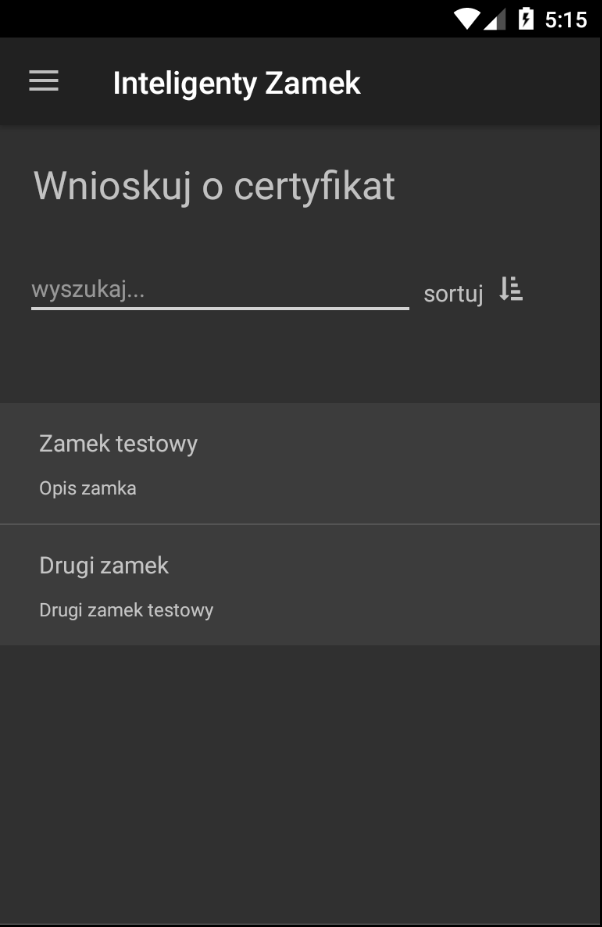
\includegraphics[width=\textwidth]
			{Obrazy/wnioskuj_o_certyfikat_pionowo}
			\caption{Panel wnioskowania o certyfikat }
			\label{rys:panel_wnioskowania_o_certyfikat_pionowo}
		\end{minipage}
		\hspace{0.1\textwidth}
		\begin{minipage}{0.45\textwidth}
			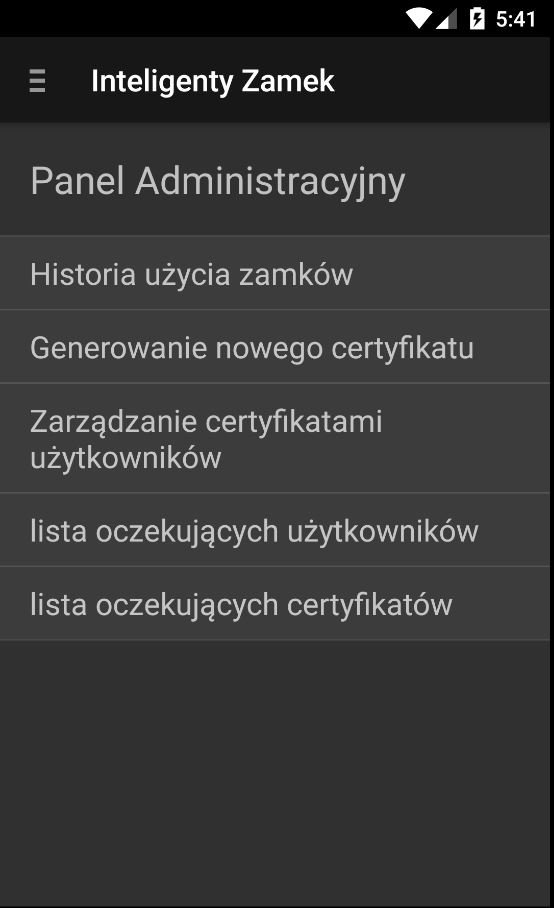
\includegraphics[width=\textwidth]{Obrazy/panel_administracyjny_pionowo}
			\caption{Panel administratora}
			\label{rys:panel_administracyjny_pionowo}
		\end{minipage}	
	\end{figure}

	\paragraph*{Panel administratora}
	W panelu administratora znajdować się będzie 6 przycisków do administrowania systemem zamków:
	\begin{itemize*}
		\item ,,Historia użycia zamków''
		\item ,,Generowanie nowego certyfikatu'',
		\item ,,Zarządzanie certyfikatami użytkowników'',
		\item ,,Lista oczekujących użytkowników do zarejestrowania'',
		\item ,,Lista oczekujących certyfikatów do zaakceptowania'',
		\item ,,Zarządzanie kontami użytkowników''.
	\end{itemize*}
	
	Po kliknięciu każdego przycisku przejdzie się do nowego odpowiadającego widoku. (Rys. \ref{rys:panel_administracyjny_pionowo})

\newpage
	
	\paragraph*{Panel historii użycia zamków}
	Panel historii użycia zamków składać się będzie z rozwijanej listy, filtrowania historii składającej się z elementów takich jak lista dostępnych zamków, lista dostępnych użytkowników, data podług której następuje filtracja oraz checkbox do zaznaczania czy tylko były nieautoryzowane próby. By uzyskać daną filtrację trzeba będzie nacisnąć przycisk filtruj. Oprócz panelu do filtrowania znajdzie się również sama historia gdzie wyświetlany jest rodzaj próby otwarcia, data oraz przez kogo była ta próba podjęta. (Rys. \ref{rys:panel_historii_uzycia_zamka_pionowo} i \ref{rys:panel_historii_uzycia_zamka_pionowo2})
	
	\begin{figure}[ht!]
		\begin{minipage}{0.45\textwidth}
			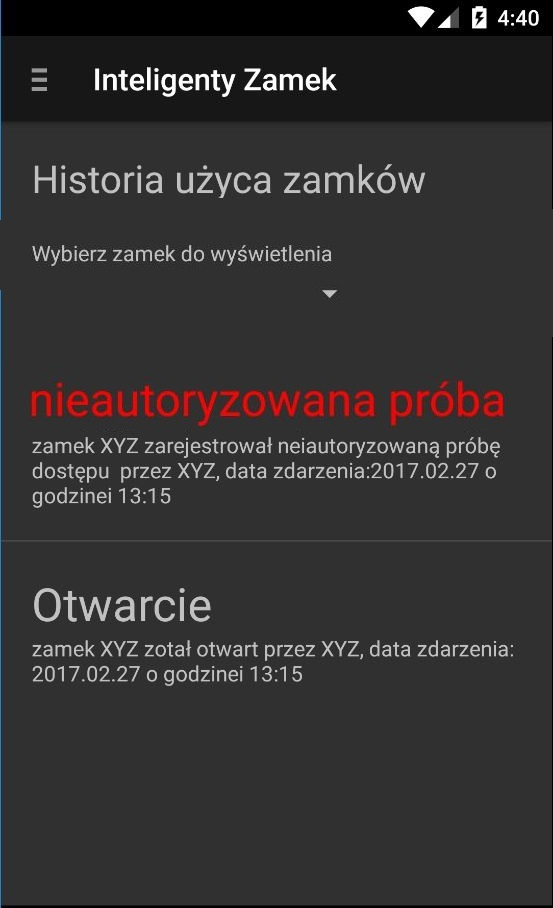
\includegraphics[width=\textwidth]{Obrazy/historia_zamkow_pionowo}
			\caption{Panel historii użycia zamków (filtr)}
			\label{rys:panel_historii_uzycia_zamka_pionowo}
		\end{minipage}
	\hspace{0.1\textwidth}
		\begin{minipage}{0.45\textwidth}
			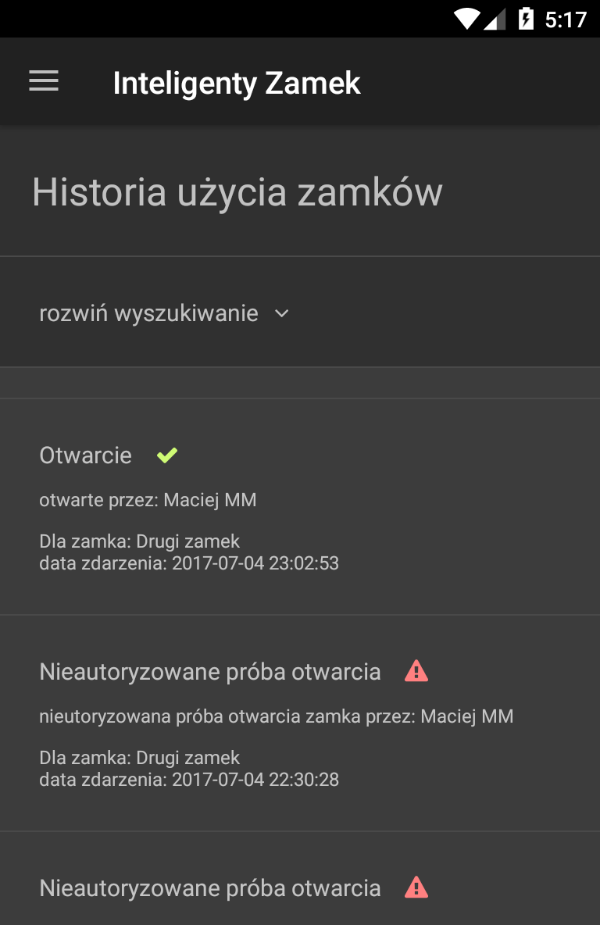
\includegraphics[width=\textwidth]{Obrazy/historia_zamkow_pionowo2}
			\caption{Panel historii użycia zamków (historia)}
			\label{rys:panel_historii_uzycia_zamka_pionowo2}	
		\end{minipage}
	\end{figure}
	\newpage
	
	\paragraph*{Panel generowania nowego certyfikatu (administrator)}
	Panel generowanie nowego certyfikatu (administrator) będzie służył do tworzenia nowych certyfikatów przez administratora. W pierwszych polach podaje się imię i nazwisko kogo dotyczy certyfikat.Następnie wybierane jest użytkownik (login) oraz zamek z rozwijanej listy. W dalszej części wybierane jest zakres dat w których certyfikat ma być ważny. Potem widać przycisk o nazwie ''zakres obowiązywania certyfikatów'', który przekierowuje do widoku odpowiedzialnego za to w jakich godzinach dla danych dni tygodni certyfikat udziela dostępu. (Rys. \ref{rys:panel_generowanie_nowego_klucza_gosc_admin_pioniowo}, \ref{rys:panel_generowanie_nowego_klucza_admin_pionowo2} i 
	\ref{rys:panel_wyboru_zakresu_certyfikatu})
	
	\vspace{-0.3cm}
	\begin{figure}[ht!]
		\begin{minipage}{0.35\textwidth}
			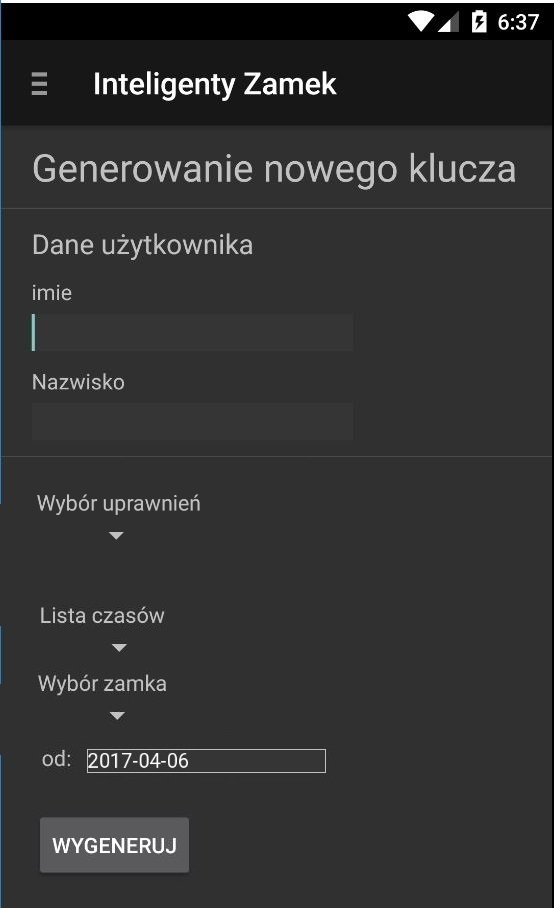
\includegraphics[width=\textwidth]{Obrazy/generowanie_nowego_klucza_gosc_admin_pioniowo}
			\caption{Panel generowania nowego klucza cz. 1 }
			\label{rys:panel_generowanie_nowego_klucza_gosc_admin_pioniowo}
		\end{minipage}
		\hspace{0.3\textwidth}
		\begin{minipage}{0.35\textwidth}
			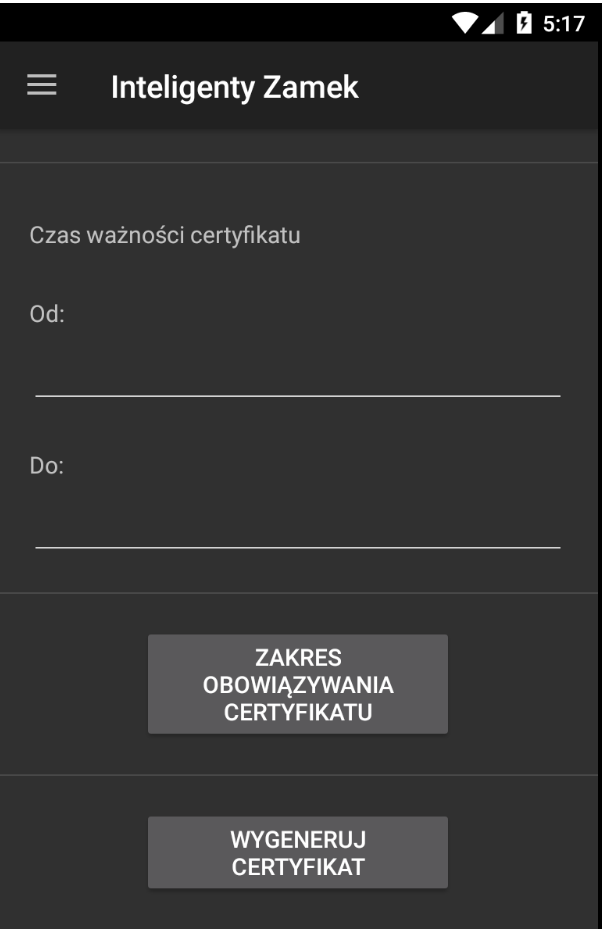
\includegraphics[width=\textwidth]{Obrazy/generowanie_nowego_klucza_admin_pionowo2}
			\caption{Panel generowania nowego klucza cz. 2}
			\label{rys:panel_generowanie_nowego_klucza_admin_pionowo2}	
		\end{minipage}
	\end{figure}
	\vspace{-0.55cm}
	\begin{figure}[ht!]
		\center
			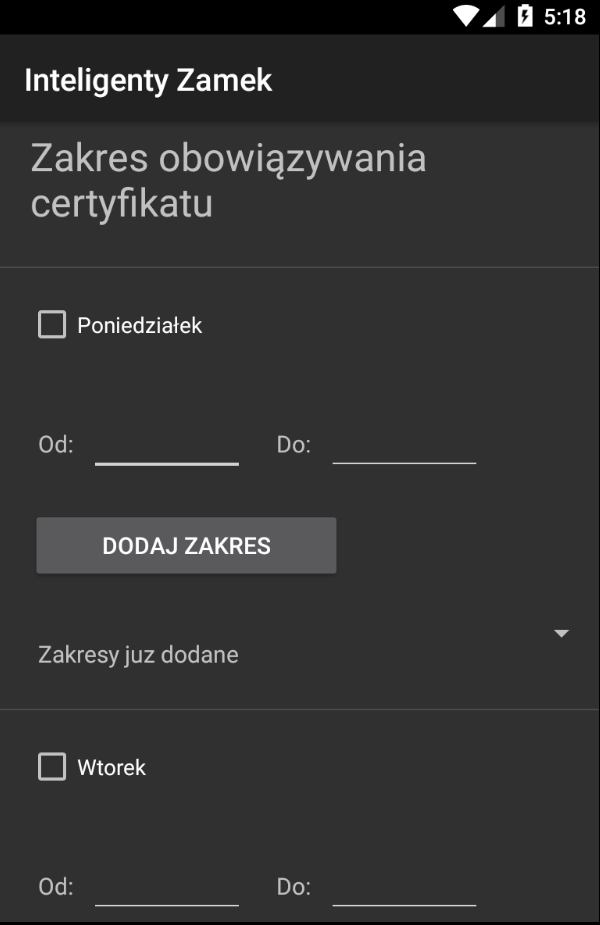
\includegraphics[width=5.8cm]{Obrazy/generowanie_nowego_klucza_uzytkownik_zalogowany_admin_pioniowo}
			\caption{Panel generowania nowego klucza cz. 3}
			\label{rys:panel_wyboru_zakresu_certyfikatu}
	\end{figure}
\newpage
	
	\paragraph*{Panel zarządzania certyfikatami~(administrator)}
	Panel zarządzania certyfikatami użytkowników (administrator) będzie widokiem tylko wszystkich aktywnych certyfikatów w systemie. Administrator klikając na pozycję przejdzie do panelu certyfikatu opisanego wyżej. Tam może usunąć dostęp lub go przedłużyć. Ułatwieniem jest możliwość wyboru typu sortowania. (Rys. \ref{rys:panel_lista_certyfikatow_administrator_pionowo})
	
	\begin{figure}[ht!]
		\begin{minipage}{0.45\textwidth}
			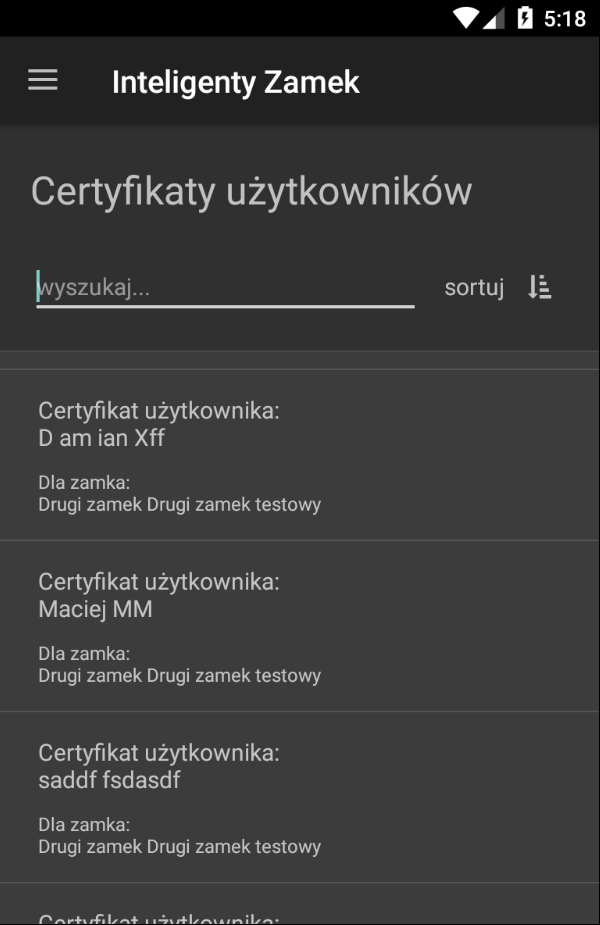
\includegraphics[width=\textwidth]{Obrazy/lista_certyfikatow_administrator_pionowo}
			\caption{Panel zarządzania certyfikatami (administrator) }
			\label{rys:panel_lista_certyfikatow_administrator_pionowo}
		\end{minipage}
		\hspace{0.1\textwidth}
		\begin{minipage}{0.45\textwidth}
			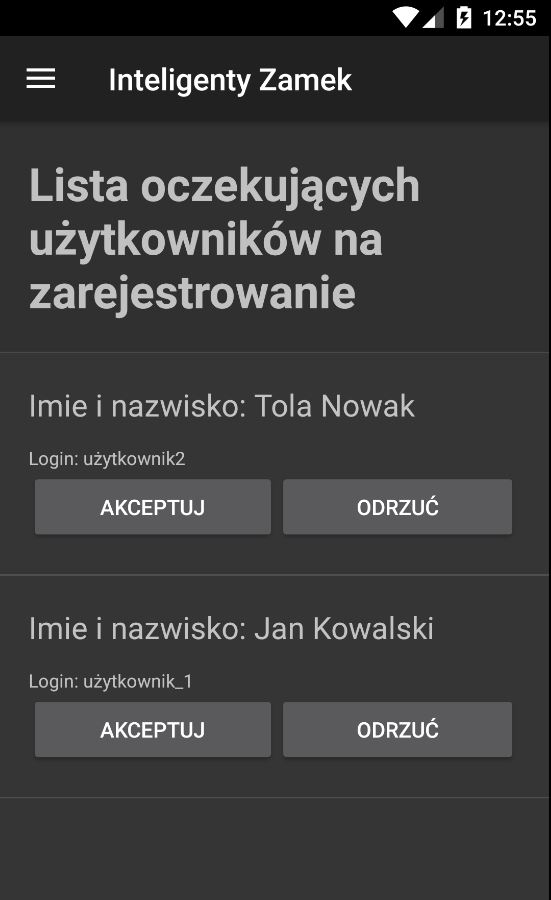
\includegraphics[width=\textwidth]{Obrazy/lista_oczekujacych_uzytkownikow_pionowo}
			\caption{Panel listy oczekujących użytkowników }
			\label{rys:panel_lista_oczekujacych_uzytkownikow_pionowo}	
		\end{minipage}
	\end{figure}
	
	\paragraph*{Panel~listy~oczekujących~użytkowników~do~rejestracji}
	Panel listy oczekujących użytkowników będzie listą wszystkich gości, którzy ubiegają się o zarejestrowanie. Po kliknięciu w odpowiednią pozycję pojawiają się dwie opcję: ''AKCEPTUJ” lub ''ODRZUĆ”.  (Rys. \ref{rys:panel_lista_oczekujacych_uzytkownikow_pionowo} )
\newpage
	
	\paragraph*{Panel~listy~oczekujących~certyfikatów do~wygenerowania}
	Panel listy oczekujących certyfikatów będzie listą wszystkich certyfikatów, które ubiegającyh się o akceptację administratora. Po kliknięciu w odpowiednią pozycję pojawią się dwie opcję: ''AKCEPTUJ” lub ''ODRZUĆ”.  (Rys. \ref{rys:panel_lista_oczekujacych_certyfikatow_pionowo} )
	
	\begin{figure}[ht!]
		\begin{minipage}{0.45\textwidth}
			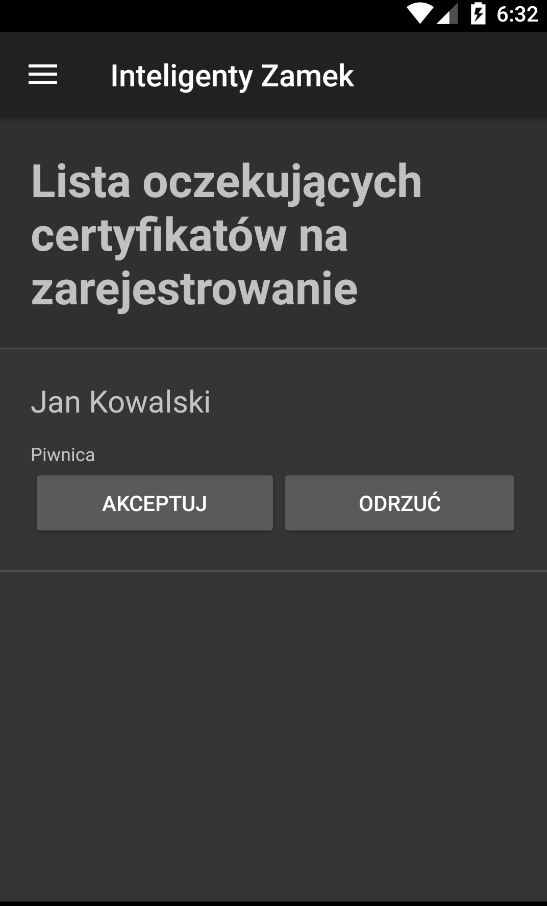
\includegraphics[width=\textwidth]{Obrazy/lista_oczekujacych_certyfikatow_pionowo}
			\caption{Panel listy oczekujących certyfikatów }
			\label{rys:panel_lista_oczekujacych_certyfikatow_pionowo}
		\end{minipage}
		\hspace{0.1\textwidth}
		\begin{minipage}{0.45\textwidth}
			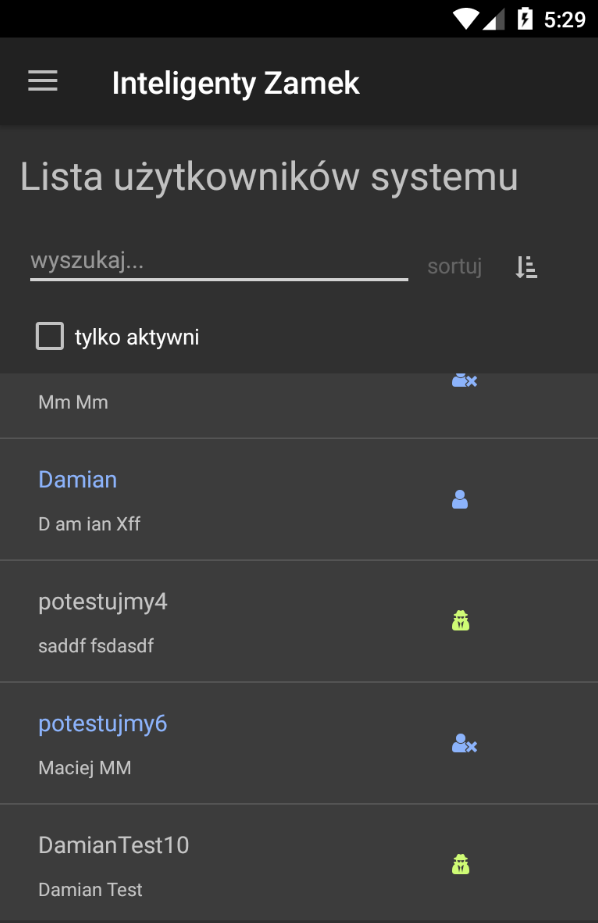
\includegraphics[width=\textwidth]{Obrazy/zarzadzanie_kontami}
			\caption{Panel zarządzania kontami użytkowników}
			\label{rys:panel_Zarządzania_Kontami}	
		\end{minipage}
	\end{figure}

	\paragraph*{Panel zarządzania kontami użytkowników}
	Panel ten służyć będzie do zarządzania kontami użytkowników. Wyświetli on listę użytkowników systemu wraz z z oznaczeniami czy jest on aktyny bądź zablokowany oraz czy ma ważny klucz szyfrujący (Rys. \ref{rys:panel_Zarządzania_Kontami})

\newpage
	
	\paragraph*{Panel ustawień konta}
	W panelu ustawień użytkownik będzie mógł zmienić hasło do swojego konta. Wymaga podania starego hasła, a następnie nowego. Ponadto w panelu tym będzie podgląd certyfikatu szyfrującego wraz z możliwością wygenerowania nowego oraz zmianę adresu ip serwera  (Rys. \ref{rys:panel_ustawienia_pionowo} i \ref{rys:panel_ustawienia_pionowo2} i \ref{rys:panel_ustawienia_pionowo3}).
	
	\begin{figure}[ht!]
		\begin{minipage}{0.35\textwidth}
			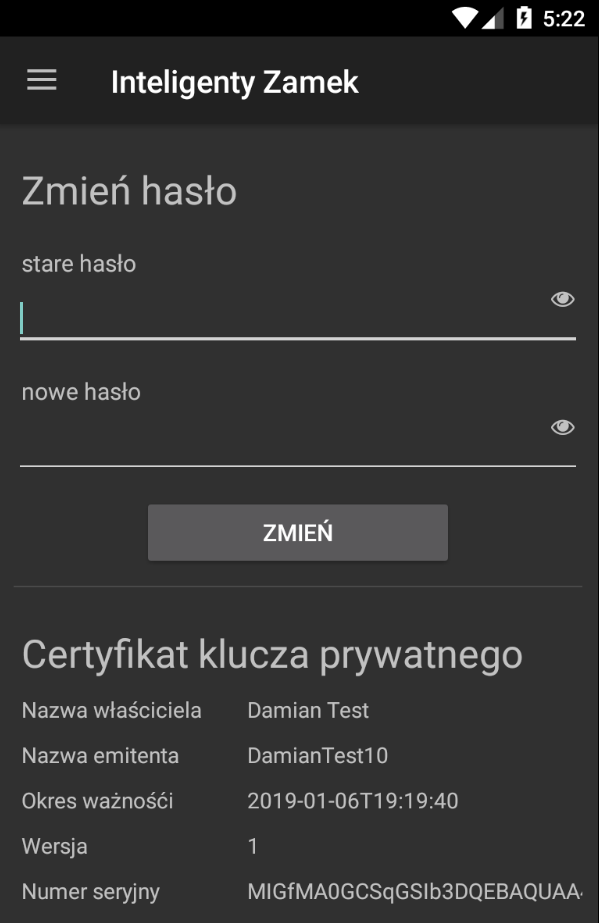
\includegraphics[width=\textwidth]{Obrazy/ustawienia_1}
			\caption{Panel generowania nowego klucza cz. 1 }
			\label{rys:panel_ustawienia_pionowo}
		\end{minipage}
		\hspace{0.3\textwidth}
		\begin{minipage}{0.35\textwidth}
			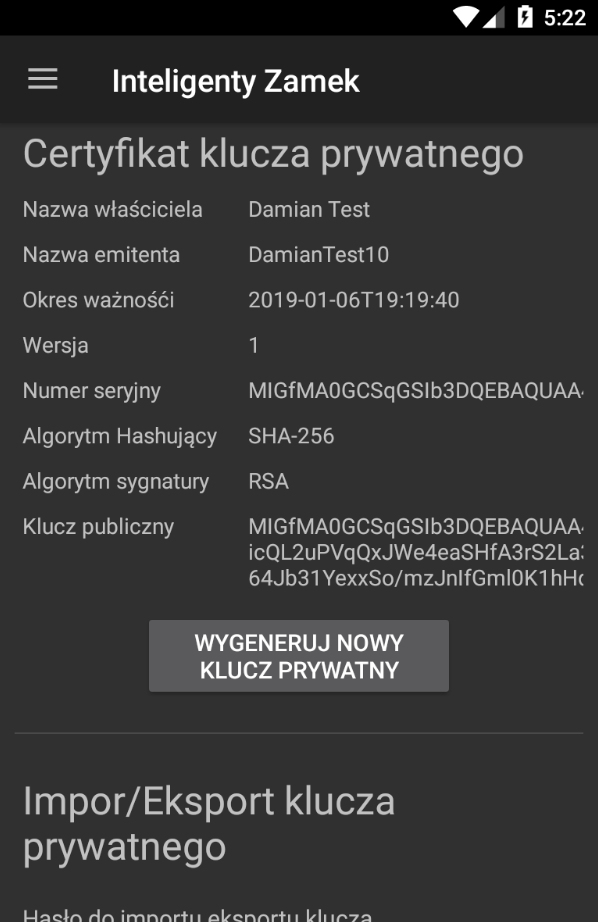
\includegraphics[width=\textwidth]	{Obrazy/ustawienia_2}
			\caption{Panel generowania nowego klucza cz. 2}
			\label{rys:panel_ustawienia_pionowo2}	
		\end{minipage}
	\end{figure}
	\begin{figure}[ht!]
			\centering
		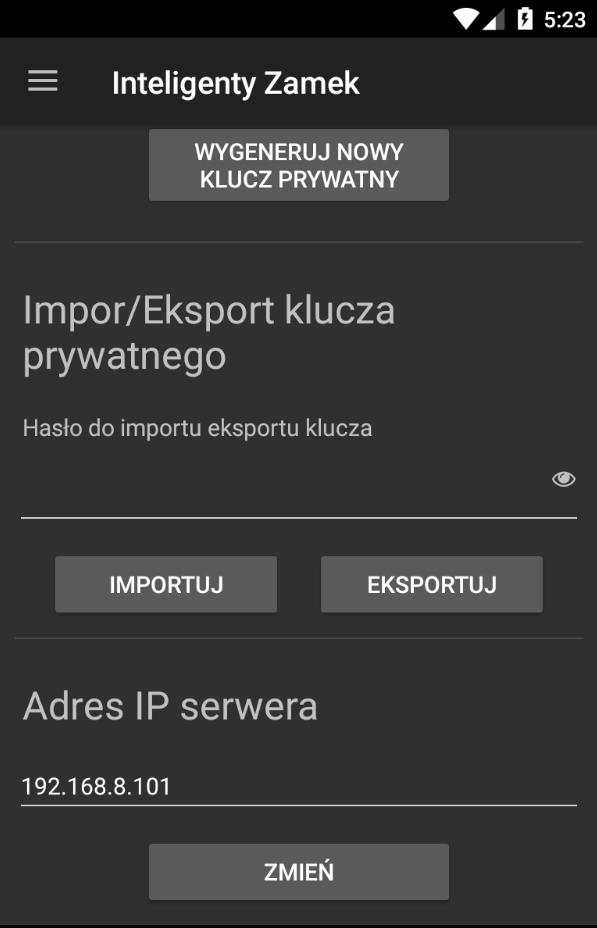
\includegraphics[width=6cm]
	{Obrazy/ustawienia_3}
	\caption{Panel ustawień konta (adres ip)}
	\label{rys:panel_ustawienia_pionowo3}
\end{figure}
	\newpage

	\subsubsection{Widoki strony internetowej systemu}
	Strona internetowa posiadać powinna dwa widoki, jeden widok logowania  (Rys. \ref{rys:strona_1}, w którym administrator musi wpisać login oraz hasło. W drugim widoku mamy listę historii otwarcia zamków  (Rys. \ref{rys:strona_2}) wraz z zaznaczeniem kolorystycznym które pokazuje czy była to próba autoryzowana.

\begin{figure}[ht!]
		\centering
	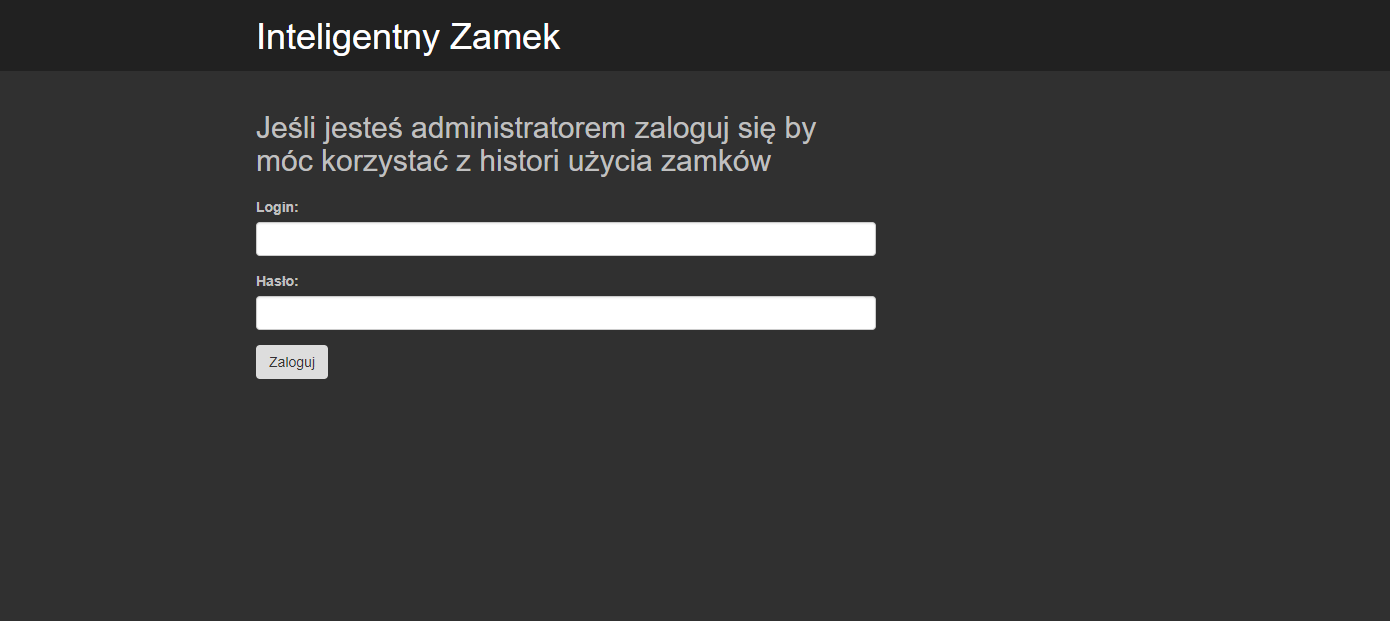
\includegraphics[width=16cm,height=10cm,keepaspectratio]
{Obrazy/strona_logowanie}
\caption{Strona logowania}
\label{rys:strona_1}
\end{figure}

\begin{figure}[ht!]
		\centering
	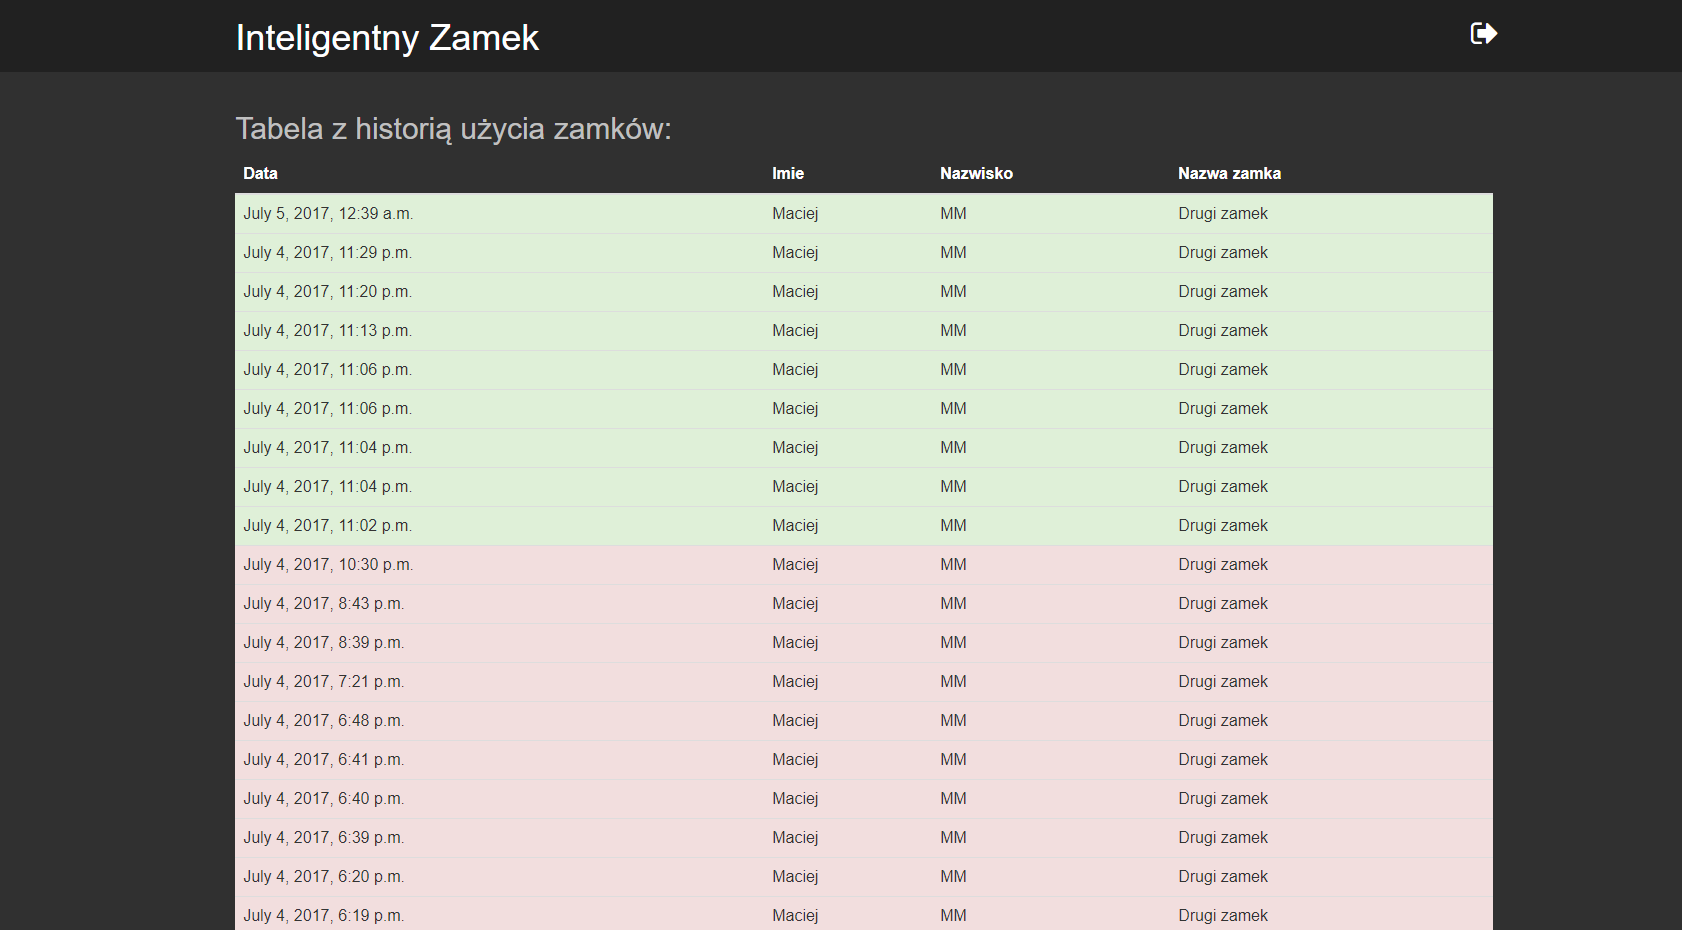
\includegraphics[width=16cm,height=10cm,keepaspectratio]
{Obrazy/strona_historia}
\caption{Strona z wyświetloną historią użycia zamków)}
\label{rys:strona_2}
\end{figure}
	\newpage
	\subsubsection{Komunikacja człowiek-interfejs}
	Aplikacja komunikować się może z człowiekiem na wiele sposób, jednym z nich są komunikaty tekstowe lub znane symbole informujące o funkcjonalności. 
		\paragraph*{Komunikaty tekstowe}
			 W aplikacji mobilnej komunikaty są wyświetlane przy pomocy toast. Komunikaty te  trwają na ekranie 4 sekundy. Informują one użytkownika o zaistniałych sytuacjach takich jak
			 \begin{itemize*}
			 	\item błąd połączenia z bazą danych
			 	\item informacja o zablokowanym koncie 
			 	\item informacja o czynnościach dodania bądź usunięcia odpowiednio użytkownika bądź certyfikatu
			 	\item o pobraniu listy certyfikatów
			 \end{itemize*}
		 
		 Dodatkowo są wyświetlane na ekranie komunikaty tekstowe przy pomocy  textview odnośnie walidacji danych oraz podpowiedzi podczas wpisywania haseł przy pomocy tooltip-ów, które informują użytkownika o parametrach jakie hasło powinno mieć.
		 
		\paragraph*{Symbolika ikon}\label{Symbolika ikon}
		Aplikacja mobilna oraz strona internetowa korzysta z symboli zawartych w fontwesome, oto poszczególne znaczenia dla danych ikon:
	  
	   	\begin{longtable}[!ht]{|m{2cm}|m{10cm}|} 
	   	\caption{Tabela ikon używanych w systemie}
	   	\label{tab:ikony}\\
	   	\hline	
	   	Ikona & Opis   \\	\hline
	   	
	  
\includegraphics[width=0.6cm]{Obrazy/full_user} 	&  	ikona oznaczająca użytkownika  aktywnego z aktualnym kluczem szyfrującym 	 
	   	\\	\hline
	   	
\includegraphics[width=0.6cm]{Obrazy/user} & 	ikona oznaczająca użytkownika  aktywnego z nieaktualnym kluczem szyfrującym \\	\hline
	   		
\includegraphics[width=0.6cm]{Obrazy/block_user}&ikona oznaczająca użytkownika zablokowanego \\	\hline
	   	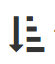
\includegraphics[width=0.6cm]{Obrazy/sort_desc}&ikonka oznaczająca sortowanie od a do z		
	   	\\	\hline				
	   	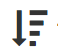
\includegraphics[width=0.6cm]{Obrazy/sort_asc}&Ikonka oznaczająca sortowanie od z do a
	   	\\	\hline
	   	
\includegraphics[width=0.6cm]{Obrazy/oko_1}	&	ikonka służąca do  pokazania na ekranie hasło które było wcześniej zamaskowane
	   	\\	\hline
	    
\includegraphics[width=0.6cm]{Obrazy/oko_2}&Ikonka służąca do maskowania hasła
	   	\\	\hline
	   	
\includegraphics[width=0.6cm]{Obrazy/menu}&Ikonka służąca do rozwijania menu
	   	\\	\hline
	   	
\includegraphics[width=0.6cm]{Obrazy/menu}&Ikonka służąca do chowania menu
	   	\\	\hline
	   	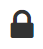
\includegraphics[width=0.6cm]{Obrazy/lock}&Ikonka oznaczająca zamknięty zamek
		\\	\hline		
	   	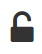
\includegraphics[width=0.6cm]{Obrazy/lock_2}&Ikonka oznaczająca otwarty zamek
	   	\\	\hline					
	   	\includegraphics[width=0.6cm]{Obrazy/error}&Ikonka oznaczająca niepoprawność np. niepoprawne hasło
	   \\	\hline
	   \includegraphics[width=0.6cm]{Obrazy/ok}& oznaczająca poprawność np. poprawny dostęp do pomieszczenia	
	   	\\	\hline							
	   \end{longtable}
	\newpage
		\paragraph*{Znaczenie kolorystyki}
		W systemie występują 4 kolory informujące użytkownika o zaistniałych sytuacjach
		\begin{itemize}
			\item czerwony który w zależności od kontekstu sugeruje albo niepoprawne wpisane dane, nie uzyskanie dostępu do pomieszczenia albo nieautoryzowaną próbę dostępu do pomieszczenia,
			\item zielony który w zależności od kontekstu sugeruje poprawne uzyskanie dostępu do pomieszczeń, autoryzowaną próbę dostępu do pomieszczenia lub użytkownika który jest aktywny, lub posiada aktualny klucz szyfrujący,
			\item żółty sugeruje w naszym systemie oczekiwanie na zdarzenie,
			\item kolor fioletowy określa użytkownika który nie ma dostępu do funkcji systemu (w zależności od ikony ma nieaktualny klucz szyfrujący lub ma konto zablokowane)
		\end{itemize}
		
	\subsubsection{Kolorystyka systemu}
	Kolorystyka systemu została oparta o styl material design, który jest dostępny dla systemu android od wersji 5.0. Strona jak i aplikacja mobilna są zbliżone kolorystycznie. Różnice w kolorach są spowodowane tylko narzuconą kolorystyką z biblioteki Bootsrap.\cite{And,desingMobile}

	\subsection{Bezpieczeństwo systemu}\label{sec:Projekt bezpieczeństwo}
	Prezentowany system ma na celu zapewniać bezpieczeństwo, zatem sam powinien być bezpieczny. Podstawowym zabezpieczeniem jakie można zastosować jest szyfrowanie połączeń oraz danych przechowywanych na nośnikach. Pierwszy sposób zapewnia wcześniej opisane w punkcie \ref{Komunikacja serwer} zastosowanie bezpiecznego protokoły Https. Druga forma zabezpieczania, mianowicie szyfrowanie odbywać się powinno głównie po stronie aplikacji mobilnej. Zdecydowano o zastosowaniu szyfrowania AES w trybie CBC, jest to wydajny algorytm, a przy tym bezpieczny (nie wykryto jak dotąd żadnych luk). Istotną kwestią bezpieczeństwa jest również weryfikacja tożsamości oraz autoryzacja w systemie.
	\subsubsection{Projekt infrastruktury klucza publicznego (PKI)}\label{sec:Projekt PKI}
	W pierwszej kolejności opisana zostanie przedstawiony projekt infrastruktury klucza publicznego (w skrócie PKI). Ideą infrastruktury klucza publicznego jest zarządzanie cyfrowymi certyfikatami i kluczami szyfrującymi dla osób, oprogramowania, urządzeń i systemów. Przy jednoczesnym zachowaniu integralności, poufności oraz dostępności.
		\paragraph*{Certyfikat szyfrujący}
		Certyfikat klucza szyfrującego ma format JSONa składającego się z następujących pól:
		\begin{itemize*}
			\item ''PUBLIC\_KEY” - wartość klucza publicznego pary kluczy dostępowych,
			\item ''Signature\_Algorithm\_Identifier'' --- algorytm szyfrujący sygnaturę,
			\item ''Validity\_period'' --- data ważności pary kluczy,
			\item ''Version'' --- wersja certyfikatu,
			\item ''Issuer\_name'' --- nazwa emitenta,
			\item ''Hash\_Algorithm'' --- algorytm funkcji skrótu,
			\item ''Serial\_number'' --- unikalna wartość dla certyfikatu,
			\item ''User\_Name'' --- imię i nazwisko użytkownika.
		\end{itemize*}
	\newpage
		Przykładowa zawartość takiego certyfikatu szyfrującego może być następująca:\\
		{\footnotesize  \{\\
			''PUBLIC\_KEY'':''MIGfMA0GCSqGSIb3DQEBAQUAA4GNADCBiQKBgQC7jik\linebreak izatJoaAnSc89HJO75BRi+IUXWBOb6yfD\&nFZd5pxEmWNXxK6sKjDLfw4XbZ\linebreak sQhBDzLAQ6KvgzNx2+WUB9nBDnP00KQ1BmvOh7GWiCeXf44Xaj3\%n+k+znM7\linebreak uRW9TpTLwOZwNpJAtec89g6UC9d+1QCH3fd950zhlYxTu21DemwIDAQAB\%n'',\\
			''Signature\_Algorithm\_Identifier'':''RSA'',\\
			''Validity\_period'':''2018-12-18T20:59:29'',\\
			''Version'':1,\\
			''Issuer\_name'':''Test10'',\\
			''Hash\_Algorithm'':''SHA-256'',\\
			''Serial\_number'':''MIGfMA0GCSqGSIb3DQEBAQUAA4GNADCBiQKBgQD\linebreak gW6H2k5BeVvGbKY81X+cvnrGOKNgCN6017fKdkGceGhFAP6ZNyPxvzjhlUS\&\linebreak /ikJRsaybUiIKP\&/lxtiheEX9hdlbY19vbrCUn3CXO\&/ILXxlYANMk1eca\linebreak UTu+VWXg5\&/GEGQ4YeNJh+au78KSnYitPMJezrN8\&/t+hkTjAFt166eDJw\linebreak IDAQAB'',\\
			''User\_Name'':''Damian Test''  \\
		\}}
								 
		\paragraph*{Urzędy certyfikujące [Maciej Marciniak]}
		W prezentowanym systemie urzędem certyfikującym może być aplikacja serwerowa posiadająca w bazie danych przy rekordach użytkownika w tabeli Users znajdować mogą się kolumny przechowujące certyfikaty szyfrujące. W ten sposób certyfikat zostanie przypisany do konkretnej osoby. Charakter systemu nie wymusza potrzeby przechowywania historii przypisanych certyfikatów do danego użytkownika, ponieważ w obiegu systemu nie powinna pojawić się sytuacja, gdzie będą podpisane dane starym kluczem, tak jak może się zdarzyć taka sytuacja przy podpisywaniu fizycznych dokumentów. Ze względu na brak potrzeby przechowywania certyfikatów unieważnionych, nowo wygenerowane certyfikaty mogą nadpisywać stare rekordy, skutkuje to oszczędnością pamięci systemu. 
		
		Urzędem rejestrującym jest tylko pośrednio aplikacja serwerowa, właściwym modułem pełniącym tę funkcję jest aplikacja mobilna z uprawnieniami administracyjnymi.
		\paragraph*{Klient systemu [Damian Filipowicz]}
		W przypadku systemu \NazwaSys \space klientem systemu będzie Aplikacja mobilna. Będzie ona odpowiedzialna za uwierzytelnianie użytkownika w systemie oraz generowanie klucza szyfrującego, który zostanie po tym fakcie wysyłany do urzędu certyfikującego. Sam klucz szyfrujący będzie tworzony w momencie rejestracji użytkownika oraz na żądanie użytkownika.\cite{PKI}
		
	\subsubsection{Poufność}
	Poufność zostanie zapewniona przy pomocy odpowiedniego przechowywania danych. Aplikacja będzie przechowywać newralgiczne dane systemu takie jak hasło użytkownika, jego token oraz klucz szyfrujący. Kluczową kwestią jest odpowiednie przechowywanie tych danych w telefonie tak, aby nie mógł nikt niepowołany ich uzyskać. Hasło przechowywane będzie w postaci zaszyfrowanego pliku, który będzie szyfrowany kluczem wszytym w oprogramowanie aplikacji za pomocą metody AES w trybie CBC. Token użytkownika oraz klucz szyfrujący będzie przechowywany jako plik w smartphonie i szyfrowany hasłem użytkownika. Dzięki temu nawet jeżeli niepowołana osoba uzyska dostęp do danych plików nie będzie w stanie ich odszyfrować w łatwy sposób.
	
	Drugim newralgicznym punktem aplikacji mobilnej będzie transmisja danych, dlatego w komunikacji pomiędzy serwerem, a urządzeniem mobilnym wykorzystany będzie protokół Https. Co uniemożliwi podsłuch danych. Pomiędzy uprzędzeniem sterującym, a telefonem komunikacja poprzez bluetooth zabezpieczona jest kluczem aplikacji. Mechanizm ten powoduje, że żadna aplikacja nie posiadająca danego kodu nie będzie w stanie połączyć się z aplikacjami prezentowanego systemu.	
	
	\subsubsection{Dostępność}
	Dzięki popularności aplikacji mobilnych prezentowany system będzie w dużym stopniu dostępny dla użytkowników. Jedynymi zagrożeniami będzie awaria sieci komputerowej, w której znajdować będzie się serwer oraz awaria sieci elektrycznej. Pierwsze jak i drugie zagrożenie będziemy redukować w postaci możliwość uzyskania dostępu do pomieszczeń w tradycyjny sposób przy pomocy kluczy (przy zastosowaniu rozwiązania z elektrozamkiem, które nie wymaga ingerencji w mechanizm oryginalny). Ponadto drugie zagrożenie będzie też redukowane przy pomocy urządzeni awaryjnego zasilania, co umożliwi funkcjonowanie systemu po zaniku napięcia w sieci elektrycznej przez określony czas.
	\subsubsection{Integralność}
	Integralność zasobów zapewniona jest dzięki pośredniczeniu aplikacji serwerowej w dostępie do bazy danych. Modyfikacje w bazie danych wprowadzić można tylko pośrednicząc przez serwer, który weryfikuje uprawnienia i filtruje możliwe odwołania do informacji, do których nie posiada użytkownik dostępu. Wprowadzać modyfikacje będzie mógł ewentualnie administrator po wcześniejszym zalogowaniu się do aplikacji zarządzającej bazą danych.